\documentclass[a4paper,12pt]{article}
\usepackage{etoolbox}
\usepackage{fullpage}
\usepackage{amsmath,amsthm,amsfonts,amssymb,amscd}
\usepackage{xcolor}
\usepackage{graphicx}
\usepackage{placeins}
\usepackage{xepersian}

\newcommand{\StudentOne}{4011262134}
\newcommand{\StudentTwo}{4011262098}
\newcommand{\NameOne}{مینا جمشیدی}
\newcommand{\NameTwo}{مبینا محمدی}
\newcommand{\ProjectName}{مستندات پروژه stack learning}


\definecolor{CustomBackground}{HTML}{1C1C1C}
\pagecolor{CustomBackground}
\color{white}


\settextfont{Vazir.ttf}[
BoldFont = Vazir-Bold.ttf, 
Path = fonts/]
\setlatintextfont{Vazir.ttf}[
BoldFont = Vazir-Bold.ttf, 
Path = fonts/]


\renewcommand{\baselinestretch}{1.2}
\let\nobreaksection\section
\renewcommand{\section}{\nobreaksection} 

\begin{document}
	

	\hrule \medskip
	\begin{minipage}{0.3\textwidth}
		\raggedright
		\small
		\NameOne \\
		\StudentOne \\
		\NameTwo \\
		\StudentTwo
	\end{minipage}
	\begin{minipage}{0.4\textwidth} 
		\centering 
		\large\bfseries
		\ProjectName \\
	\end{minipage}
	\begin{minipage}{0.3\textwidth}
		\raggedleft
		\small
	\end{minipage}
	\medskip\hrule 
	\vspace*{1.5cm}  
	
\section{نتایج فاز اول: استخراج ویژگی و طبقه‌بندی ابتدایی}


در این بخش، عملکرد مدل‌های طبقه‌بندی مختلف بر پایه سه سطح متفاوت از ویژگی‌های استخراج‌شده از مدل \lr{ResNet18} مورد ارزیابی قرار گرفت. ویژگی‌ها به سه دسته تقسیم شدند: ویژگی‌های سطح پایین (تا لایه \lr{maxpool})، ویژگی‌های میانی (تا پایان \lr{layer2}) و ویژگی‌های سطح بالا (تا لایه \lr{avgpool}). برای هر سطح، شش مدل طبقه‌بندی مختلف شامل \lr{SVM}، \lr{KNN}، \lr{Random Forest}، \lr{Logistic Regression}، \lr{Extra Trees} و \lr{Gaussian NB} آموزش داده شدند و دقت آن‌ها روی مجموعه داده‌ی آزمایشی بررسی شد.

\vspace{0.5cm}
\textbf{۱. ویژگی‌های سطح پایین \lr{(Low-Level Features)}:}

در این سطح، ویژگی‌ها شامل لبه‌ها، الگوهای ابتدایی و اطلاعات بافتی پایه هستند. نتایج نشان دادند که این ویژگی‌ها در تفکیک کلاس‌ها محدودیت دارند. دقت بهترین مدل (\lr{Logistic Regression}) برابر با \lr{71\%} روی داده‌های آزمایشی بود. کلاس \lr{horses} به طور قابل توجهی بهتر از \lr{cats} و \lr{dogs} طبقه‌بندی شد که نشان‌دهنده‌ی تمایز بیشتر این کلاس در ویژگی‌های سطح پایین است.
\begin{figure}[h]
	\centering
	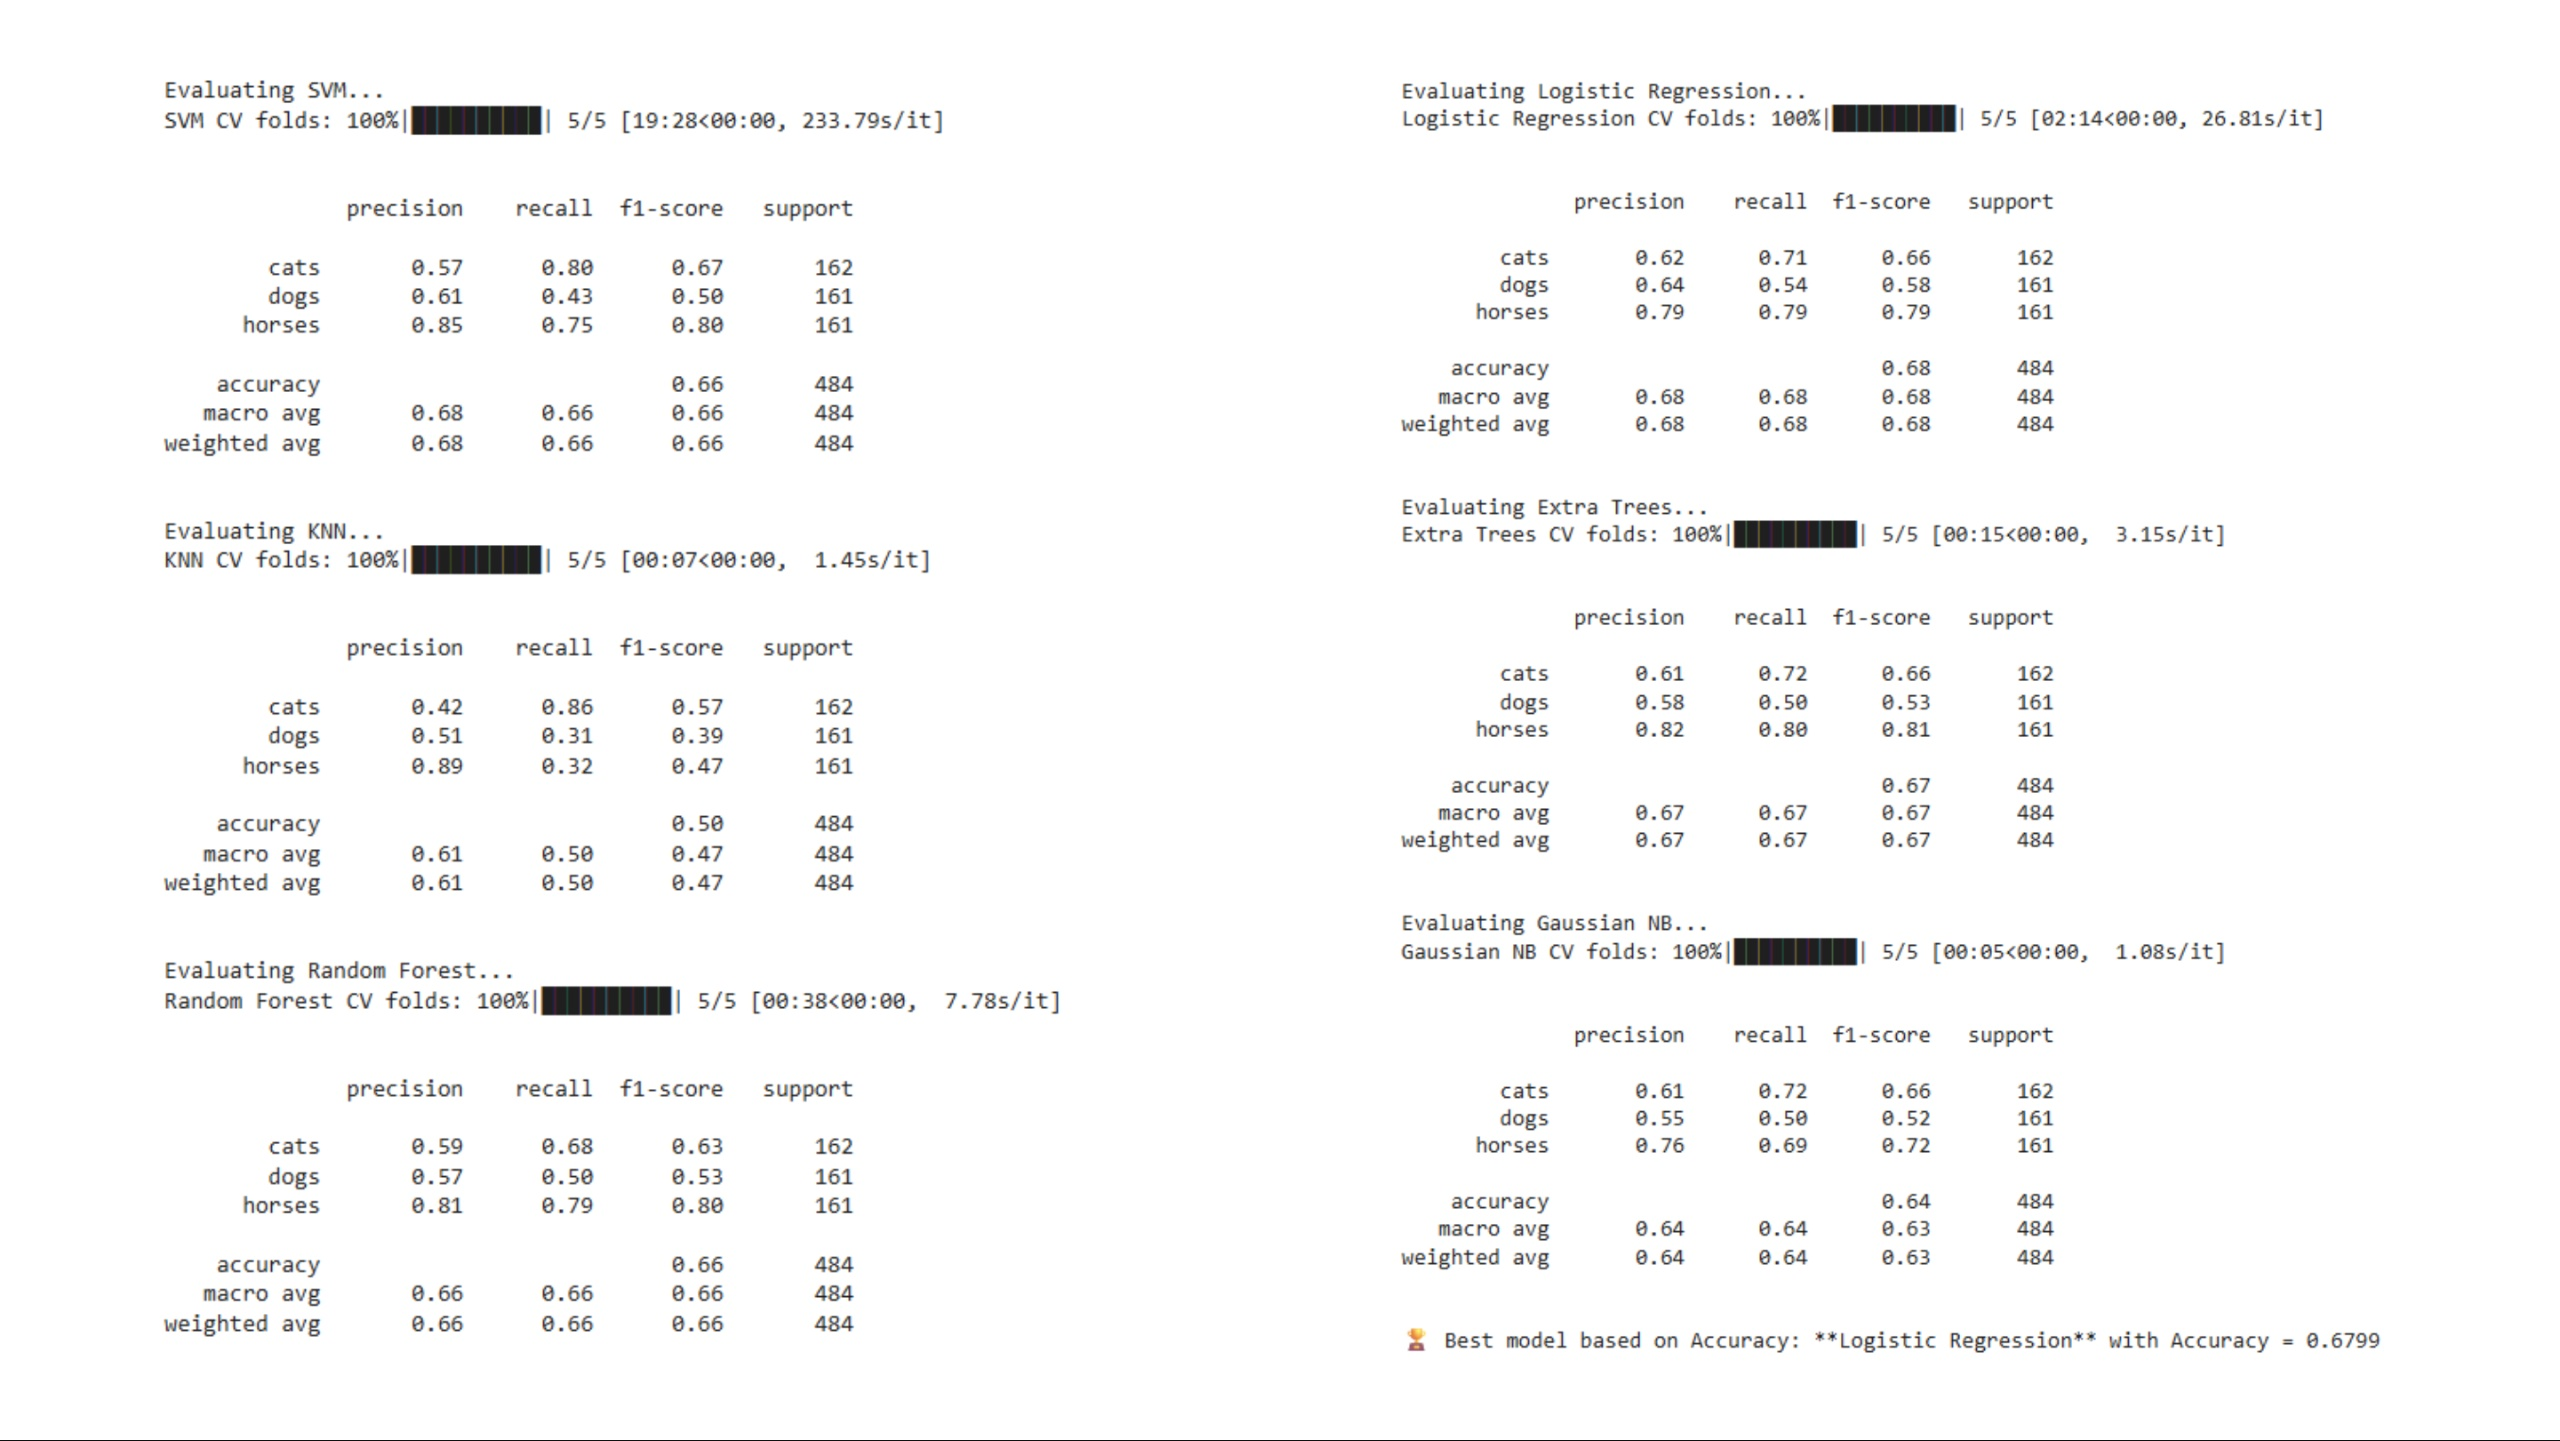
\includegraphics[width=1\textwidth]{1-1.jpg}
\end{figure}
\FloatBarrier
\begin{figure}[h]
	\centering
	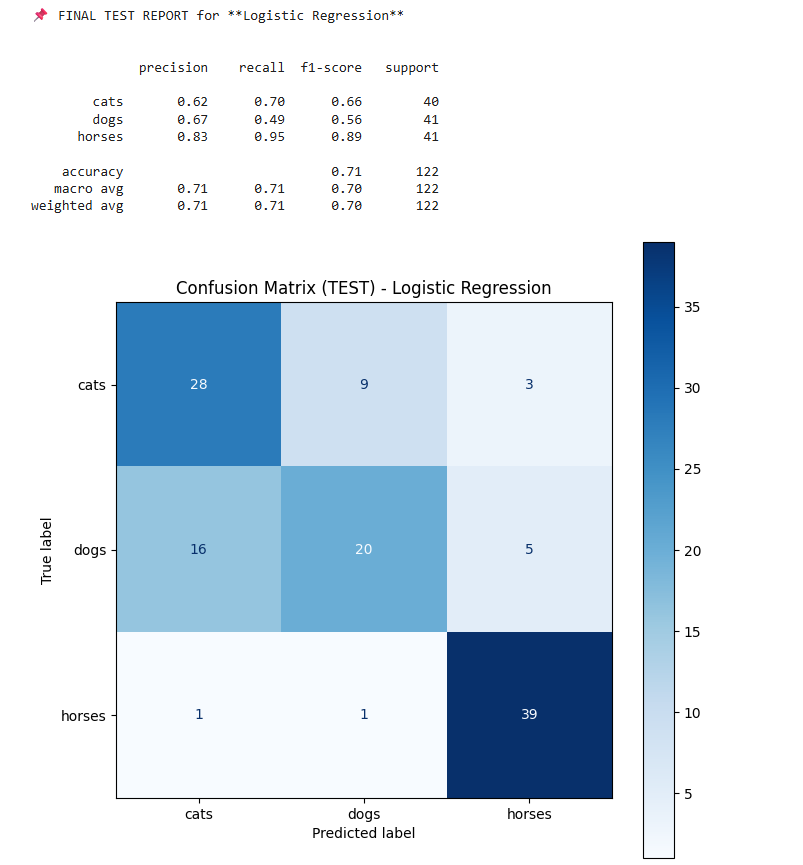
\includegraphics[width=1\textwidth]{1-2.png}
\end{figure}
\FloatBarrier

\textbf{۲. ویژگی‌های میانی \lr{(Mid-Level Features)}:}

با استفاده از لایه‌های \lr{layer1} و \lr{layer2}، مدل قادر به استخراج ویژگی‌های ترکیبی و ساختاریافته‌تری شد. در این مرحله، دقت مدل \lr{Logistic Regression} به حدود \lr{85\%} افزایش یافت و کلاس‌ها به صورت متوازن‌تری طبقه‌بندی شدند. نسبت به مرحله‌ی قبل، کلاس \lr{dogs} که پیش‌تر عملکرد ضعیفی داشت، بهبود محسوسی در دقت و \lr{recall} نشان داد. این موضوع حاکی از قدرت بیشتر ویژگی‌های میانی در بازنمایی ساختارهای مفهومی‌تر تصویر است.

\begin{figure}[h]
	\centering
	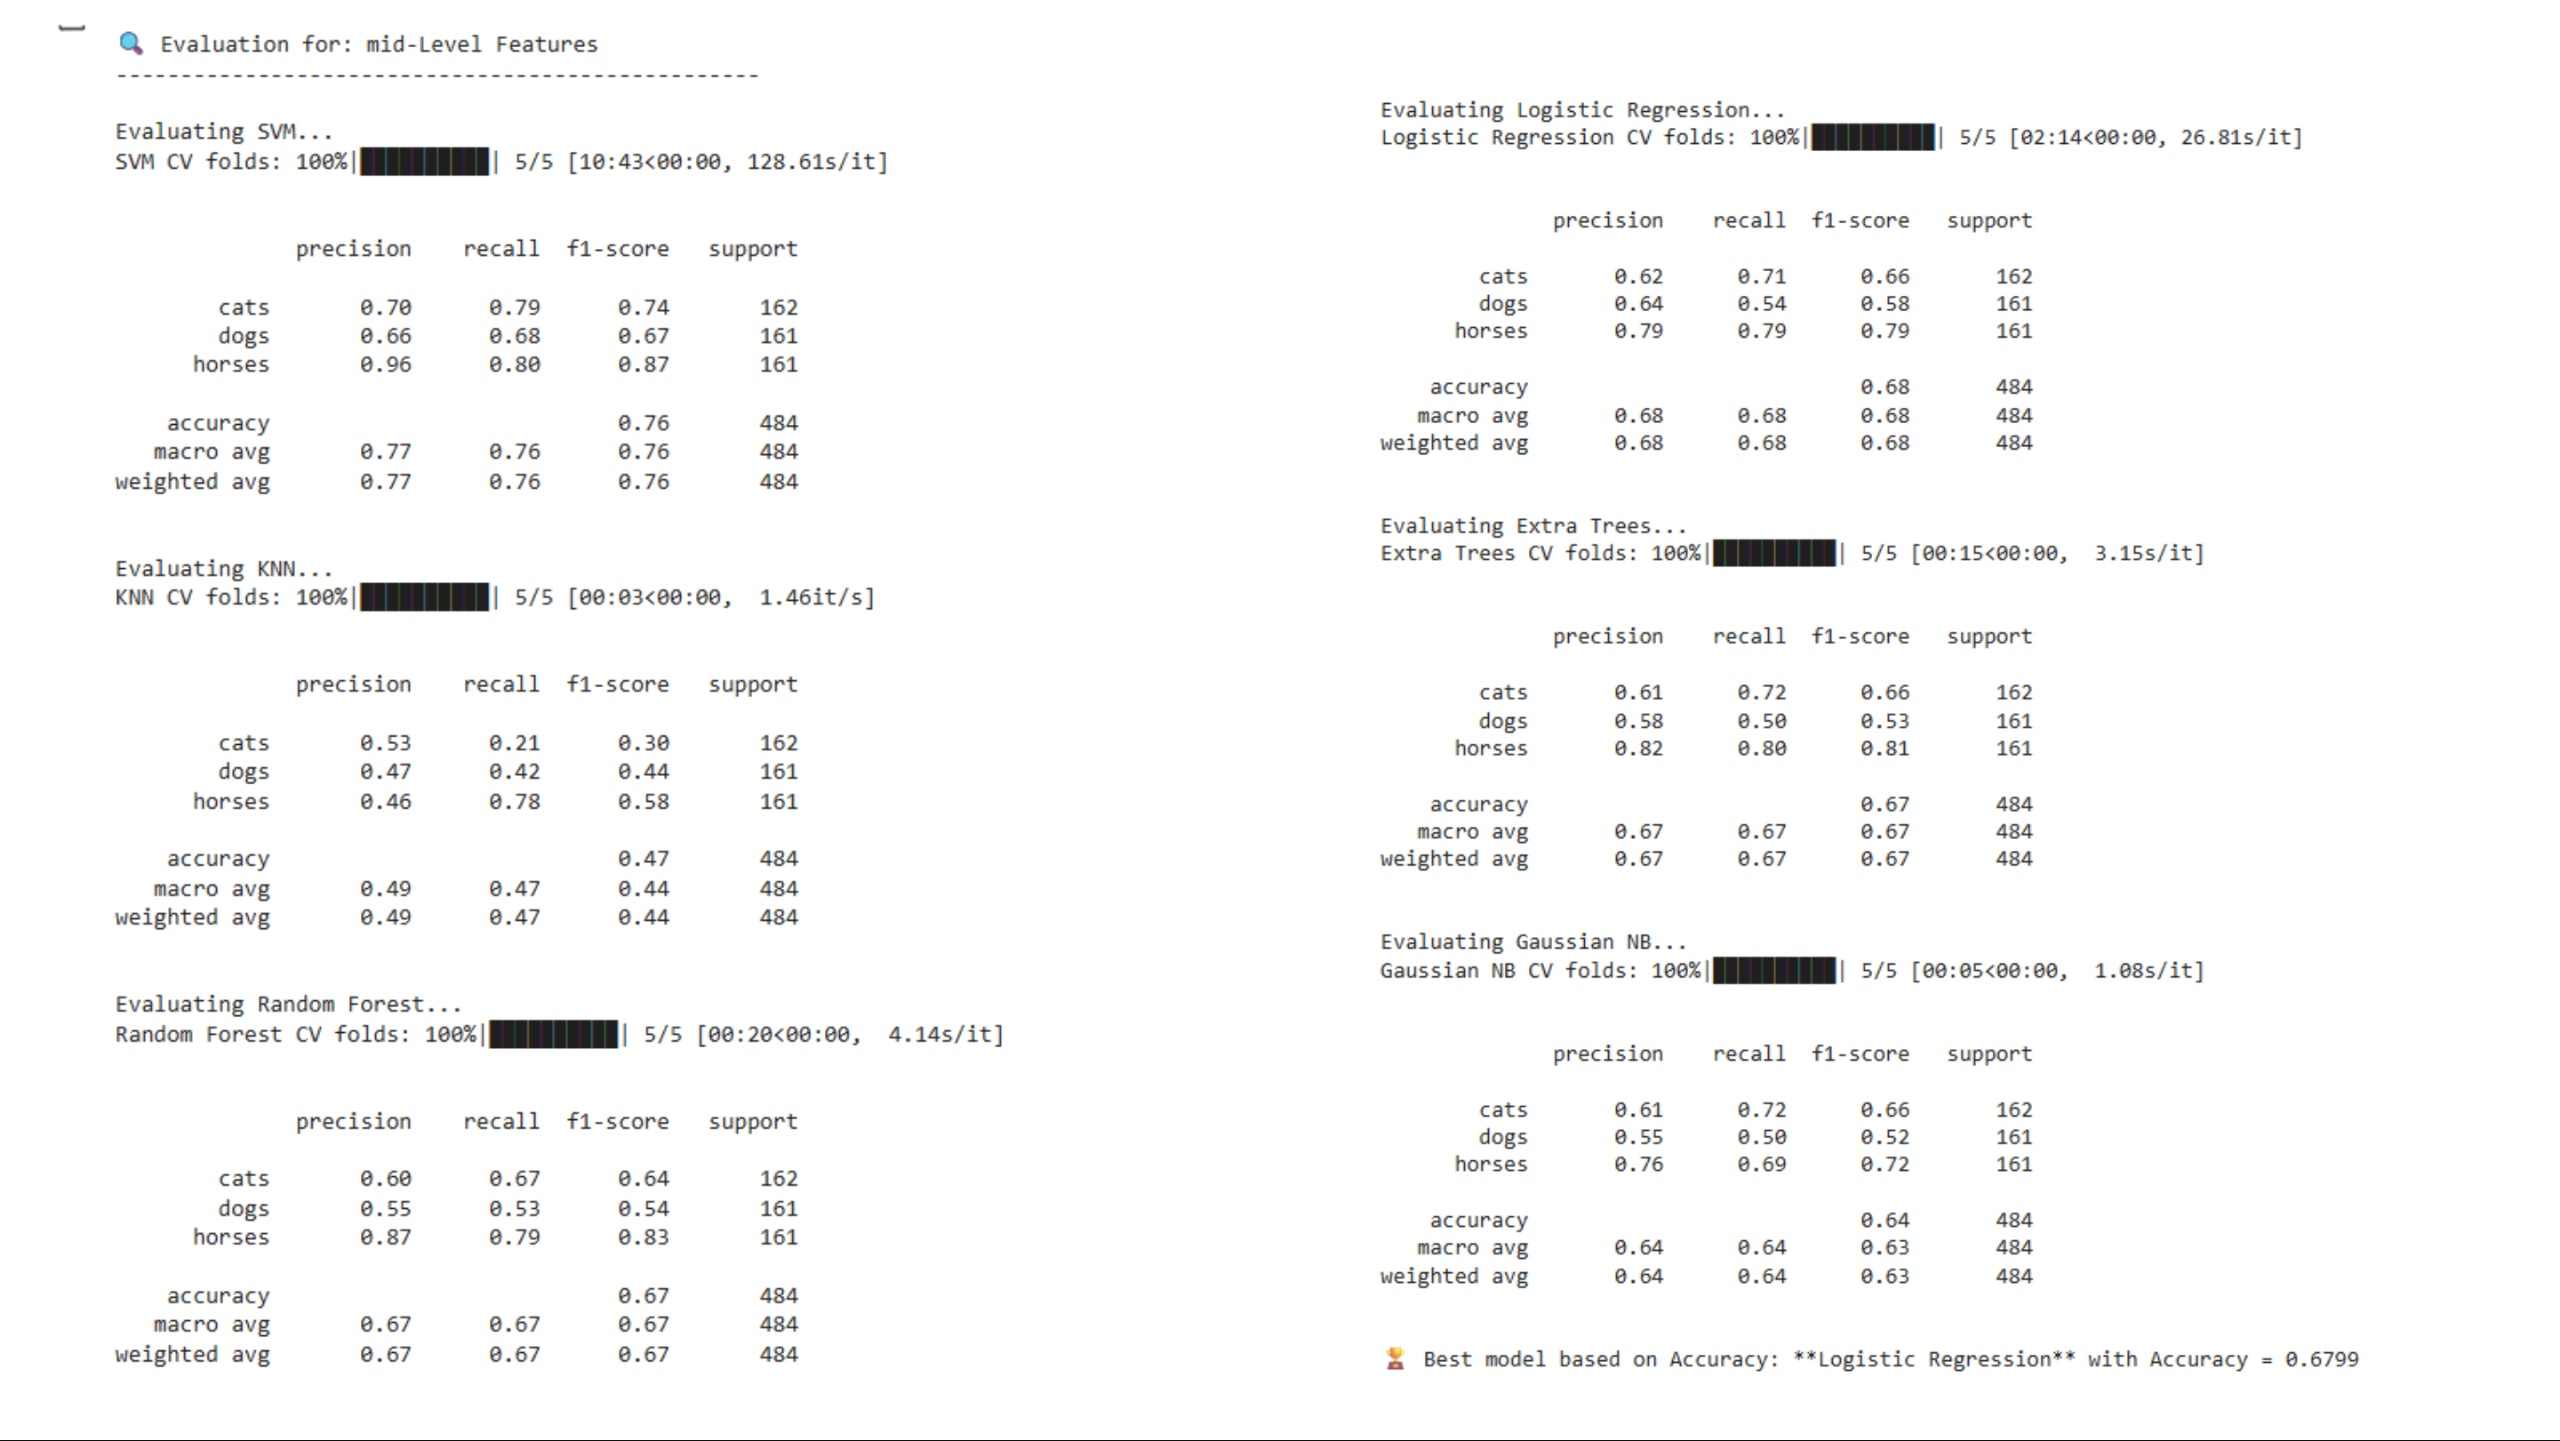
\includegraphics[width=1\textwidth]{2-1.jpg}
\end{figure}
\FloatBarrier
\begin{figure}[h]
	\centering
	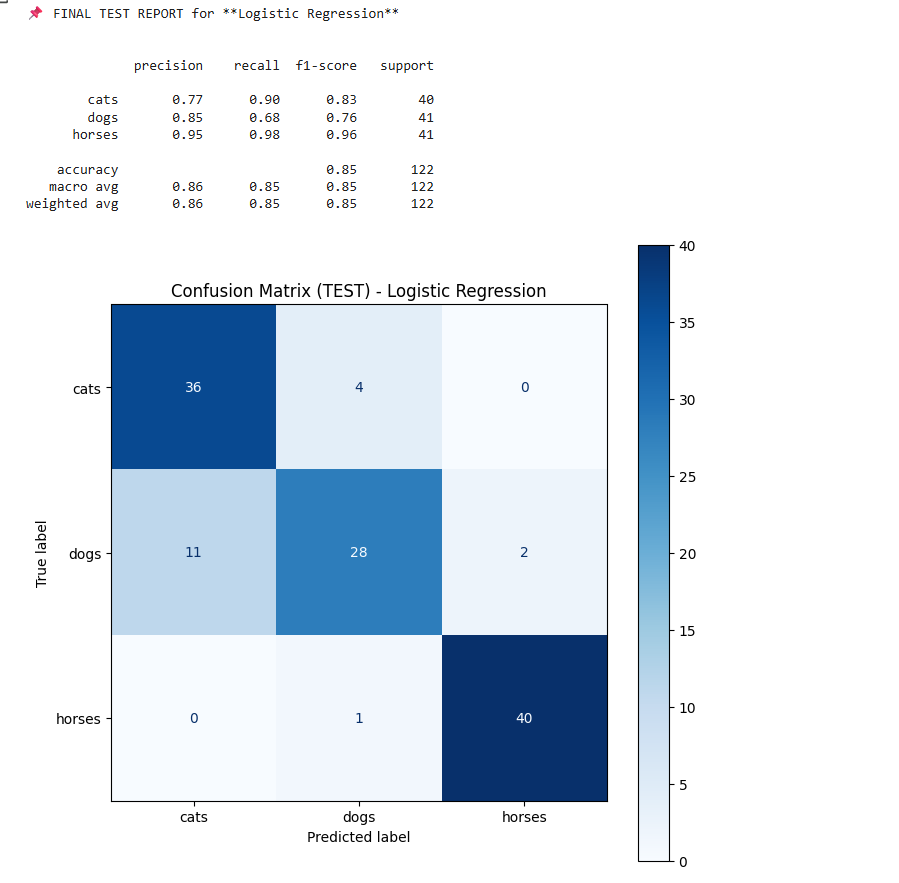
\includegraphics[width=1\textwidth]{2-2.png}
\end{figure}
\FloatBarrier

\textbf{۳. ویژگی‌های سطح بالا \lr{(High-Level Features)}:}

در این حالت، از تمام شبکه (به جز لایه FC نهایی) برای استخراج ویژگی استفاده شد. این ویژگی‌ها شامل نمایش‌های انتزاعی از مفاهیم بصری مانند "چهره گربه" یا "پیکربندی بدن اسب" هستند. مدل \lr{SVM} در این مرحله با دقت \lr{100\%} روی داده‌ی تست بهترین عملکرد را نشان داد. تمامی کلاس‌ها بدون خطا شناسایی شدند. این نتیجه تأییدی بر قدرت بالای نمایش‌های سطح بالا در مدل‌های یادگیری عمیق برای تفکیک دقیق بین کلاس‌ها است.

\begin{figure}[h]
	\centering
	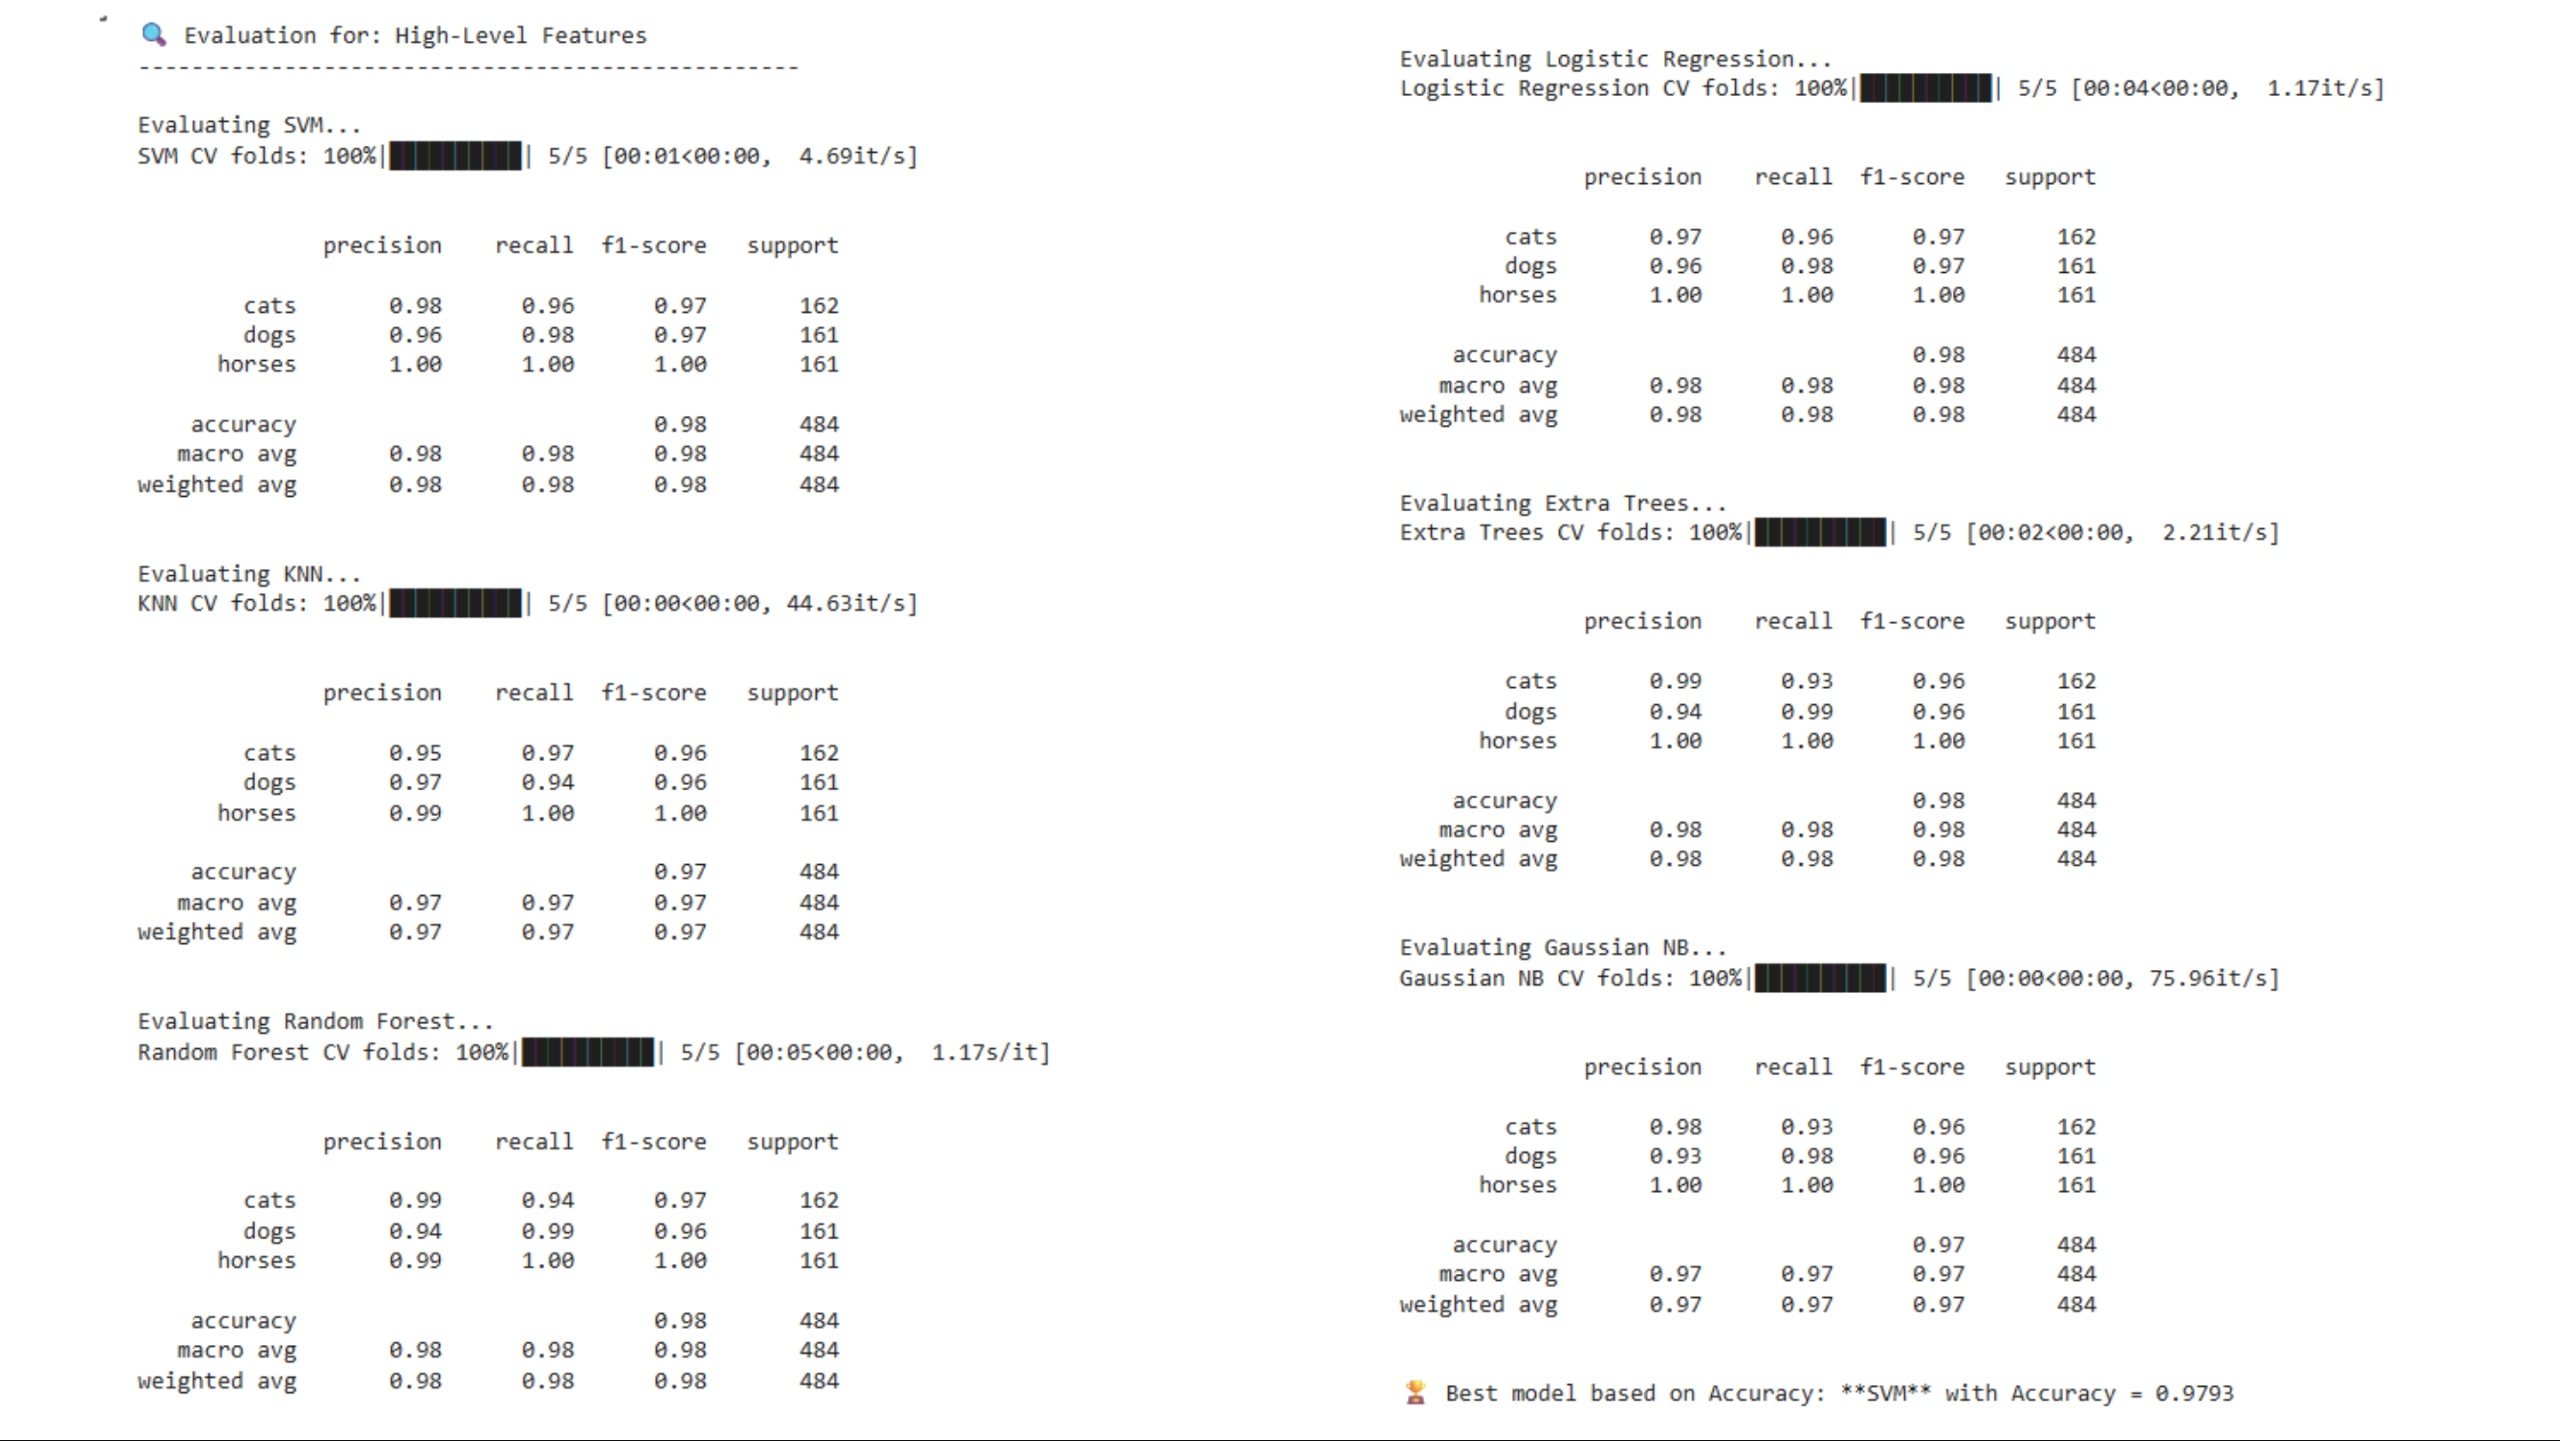
\includegraphics[width=1\textwidth]{3-1.jpg}
\end{figure}
\FloatBarrier
\begin{figure}[h]
	\centering
	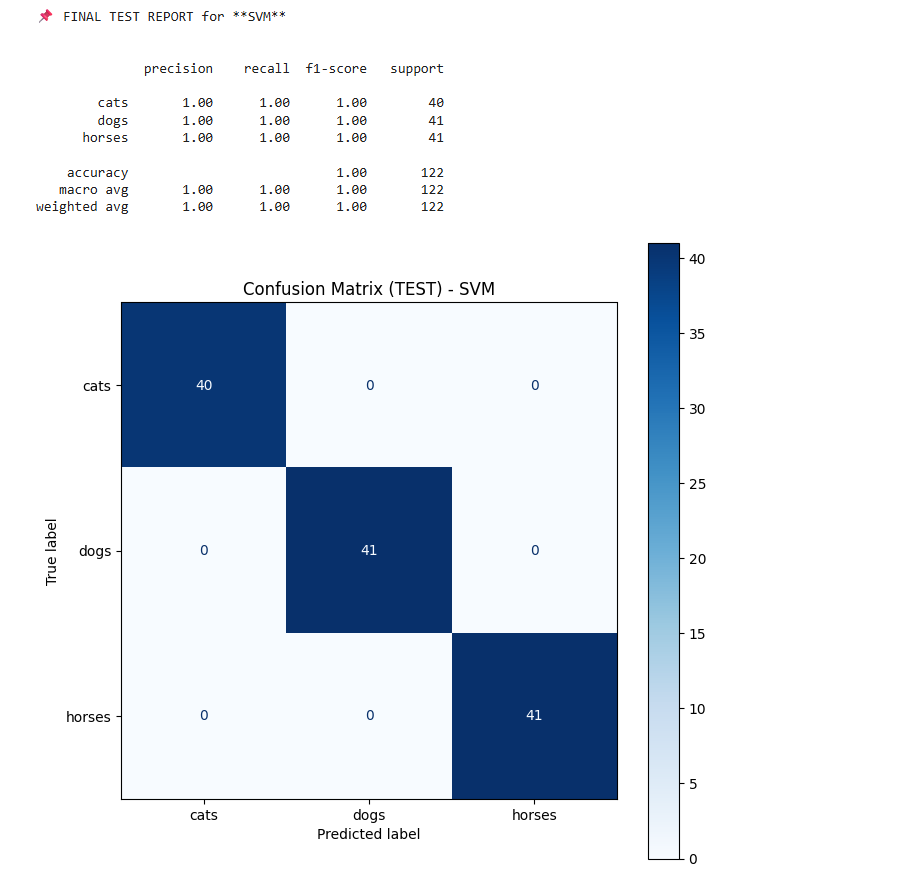
\includegraphics[width=1\textwidth]{3-2.png}
\end{figure}
\FloatBarrier
\vspace{0.5cm}
\textbf{جمع‌بندی:}

\begin{itemize}
	\item با افزایش عمق ویژگی‌های استخراج‌شده، دقت و کیفیت طبقه‌بندی نیز به‌طور قابل توجهی افزایش یافت.
	\item مدل \lr{Logistic Regression} در دو سطح اول بهترین عملکرد را داشت، در حالی که در سطح سوم، مدل \lr{SVM} با اختلاف واضحی بهترین بود.
	\item کلاس \lr{horses} در تمامی سطوح نسبت به دو کلاس دیگر بهتر طبقه‌بندی شد، که می‌تواند به تفاوت‌های بصری بارزتر این کلاس نسبت داده شود.
	\item نتایج نشان می‌دهند که حتی بدون \lr{fine-tuning} شبکه، استفاده از ویژگی‌های استخراج‌شده از \lr{ResNet18} می‌تواند عملکرد بالایی در طبقه‌بندی تصاویر داشته باشد.
\end{itemize}

\section{نتایج فاز دوم}
در این فاز، هدف ما استفاده از روش Stacking برای ترکیب خروجی مدل‌های مختلف است تا با بهره‌گیری همزمان از سطوح مختلف ویژگی‌ها (Low، Mid، High) و مدل‌های متنوع یادگیری ماشین، عملکرد نهایی طبقه‌بندی را بهبود ببخشیم. انتظار داریم این روش در مقایسه با فاز قبلی (استفاده مجزای هر مدل بر روی یک سطح از ویژگی‌ها)، نتایج بهتری به همراه داشته باشد.
\\
برای پیاده‌سازی استک لرنر، دو رویکرد متفاوت مورد استفاده قرار گرفت:
\\
۱. روش مبتنی بر کتابخانه (استفاده از StackingClassifier)\\
در این روش، از کلاس StackingClassifier در کتابخانه scikitlearn استفاده شد. مدل‌های پایه به‌صورت زیر تعریف شدند:\\
SVM \\
\lr{Random Forest}\\
\lr{Logistic Regression}\\
\lr{Naive Bayes}
\lr{MLP }\\
با استفاده از تنظیم هایپرپارامترها و آزمون مدل‌های مختلف، سعی کردیم بهترین ترکیب ممکن را برای استک بیابیم. همچنین حذف و اضافه کردن مدل‌های مختلف نیز انجام شد. این آزمایش‌ها نشان دادند که افزودن مدل‌های بیشتر به‌صورت قابل‌توجهی دقت را افزایش نمی‌دهد و صرفاً موجب افزایش زمان آموزش می‌گردد.\\
با این‌که دقت آموزش بسیار بالا بود، اما در داده‌های آزمون شاهد افت بودیم. این مسئله نشان‌دهنده وقوع Overfitting بود. برای رفع این مشکل، از  DataAugmentation استفاده شد که تا حدی در کاهش اورفیت مؤثر واقع شد، اما به سطح رضایت‌بخشی نرسید.
\\
بدون اضافه کردن داده:
\\
\begin{figure}[h]
	\centering
	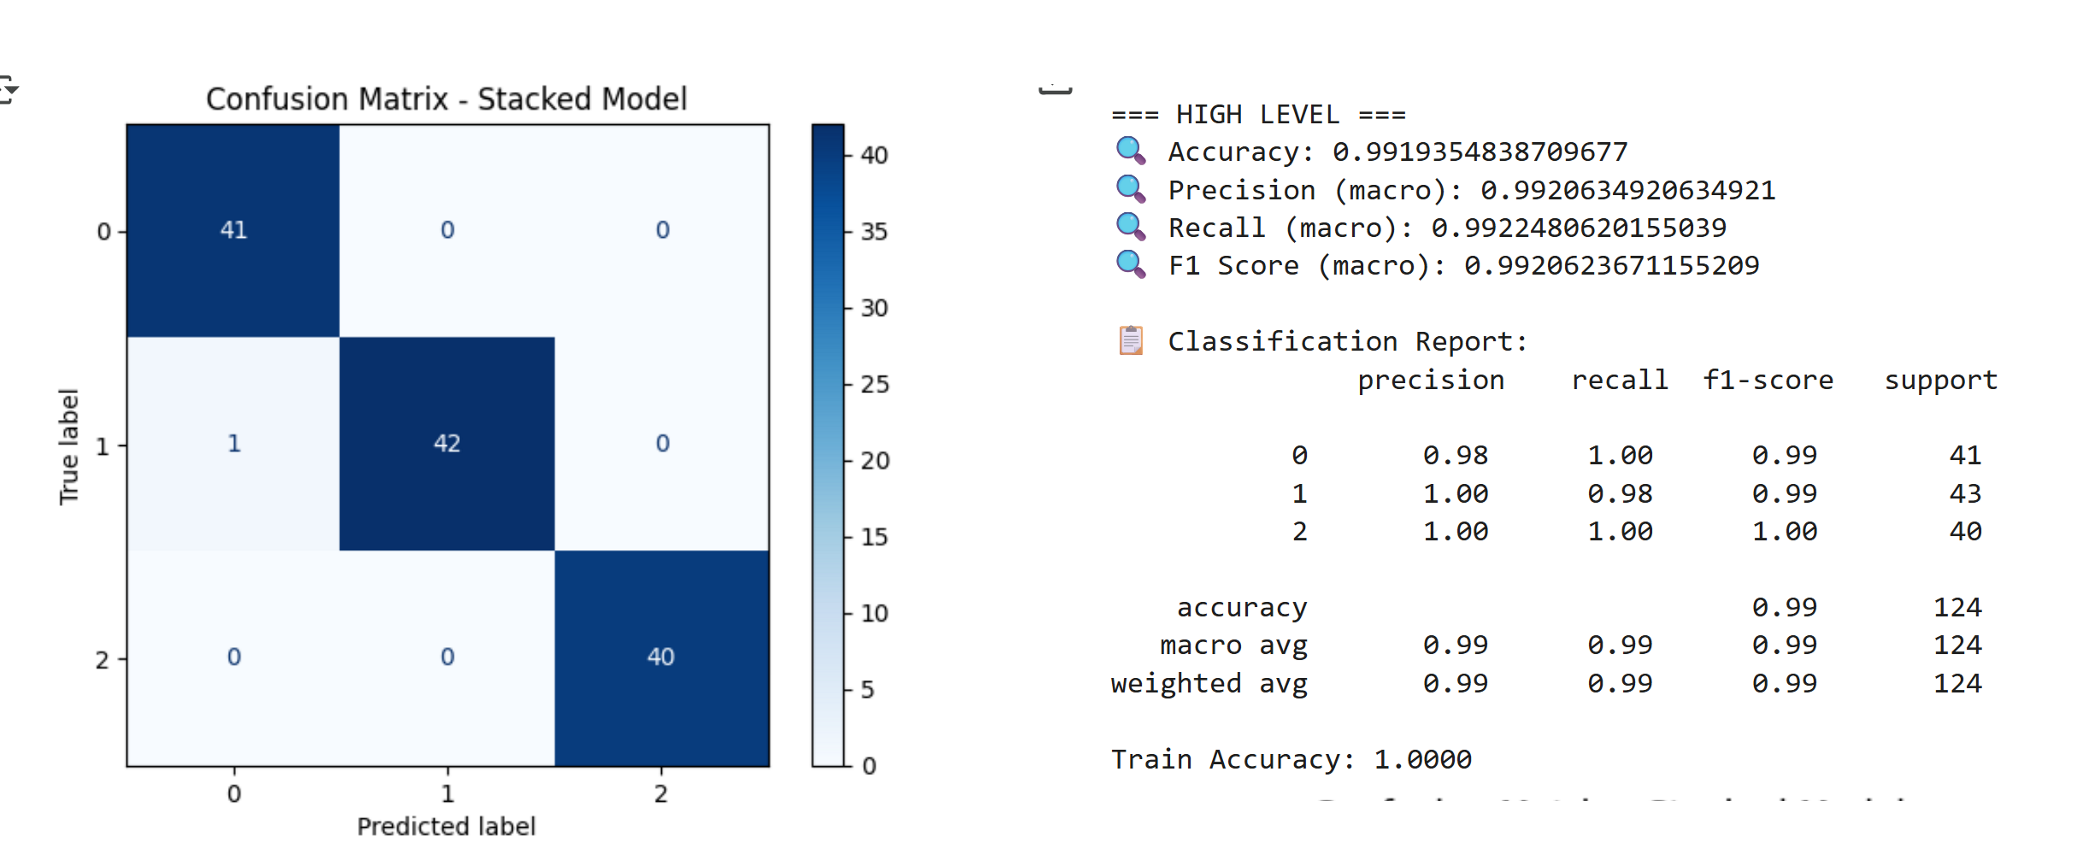
\includegraphics[width=1\textwidth]{1-high.png}
\end{figure}
\FloatBarrier
\begin{figure}[h]
	\centering
	\includegraphics[width=1\textwidth]{1-high2.png}
\end{figure}
\FloatBarrier
\begin{figure}[h]
	\centering
	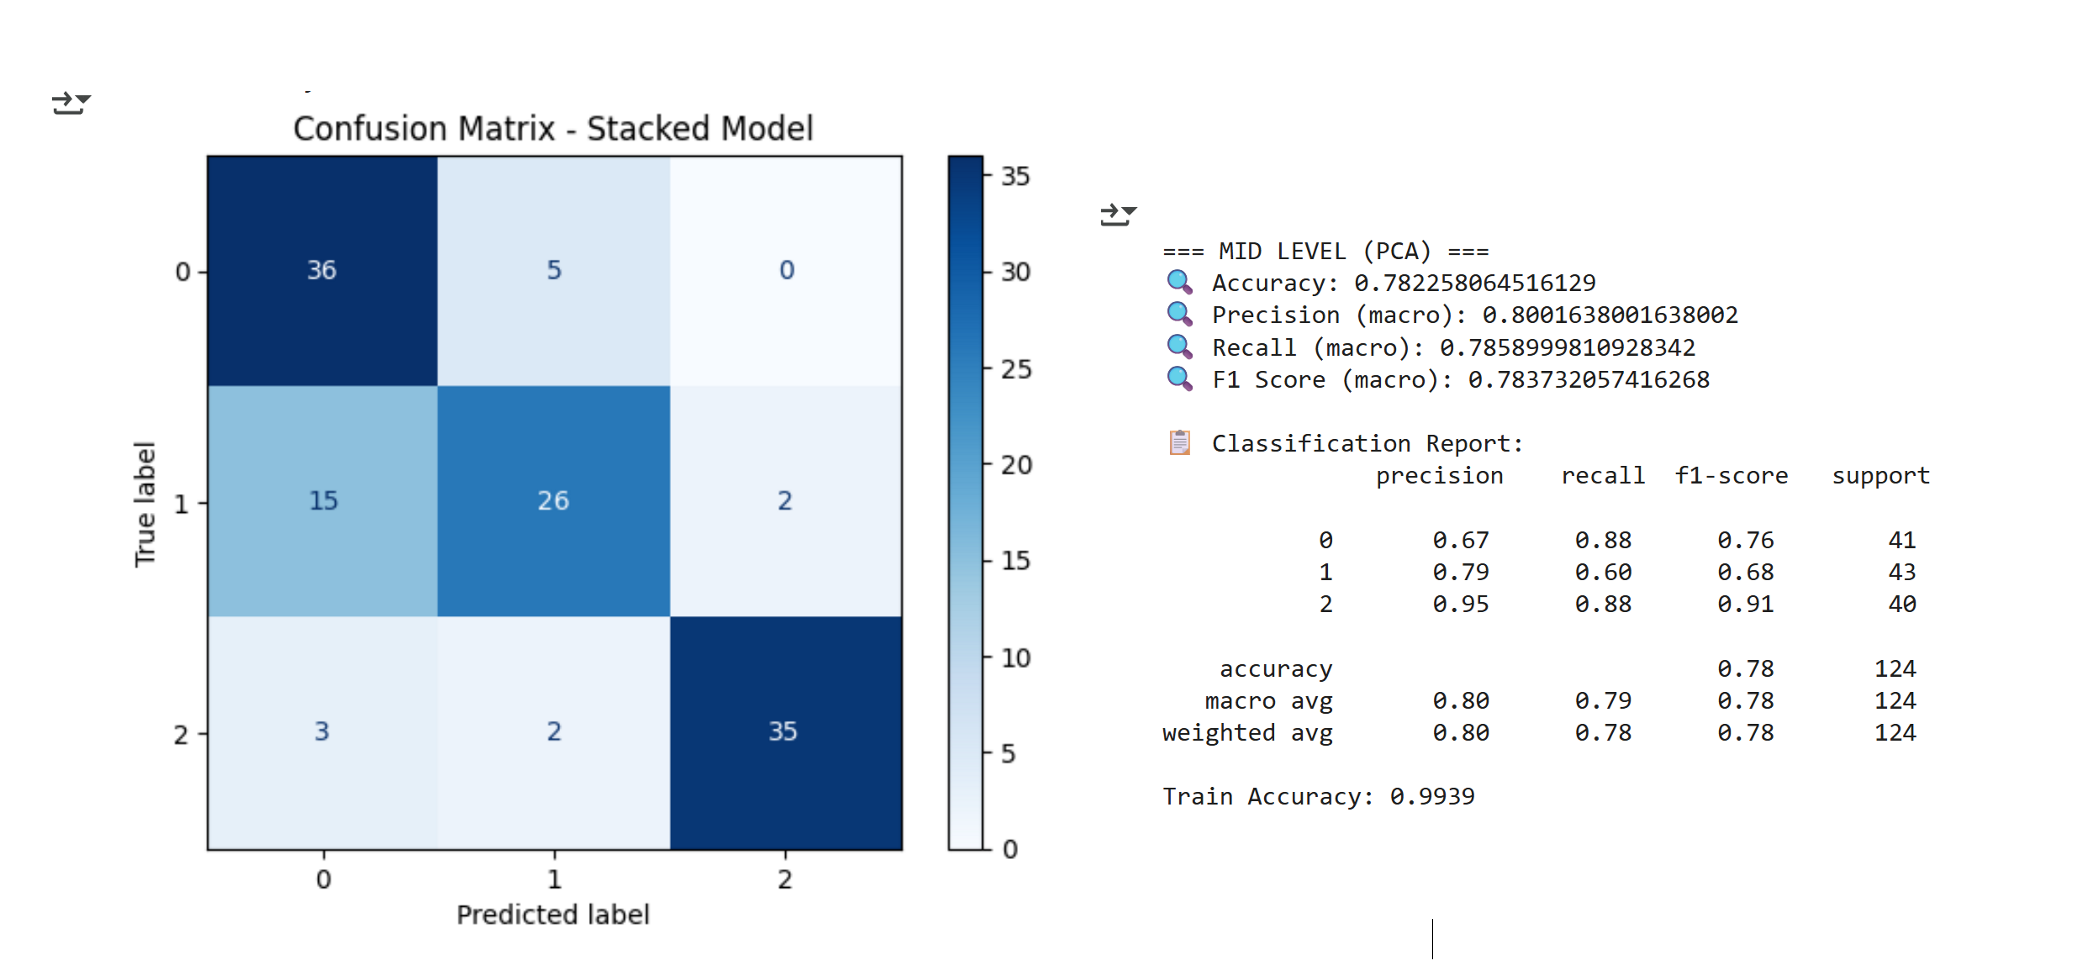
\includegraphics[width=1\textwidth]{1-mid.png}
\end{figure}
\FloatBarrier
\begin{figure}[h]
	\centering
	\includegraphics[width=1\textwidth]{1-mid2.png}
\end{figure}
\FloatBarrier
\begin{figure}[h]
	\centering
	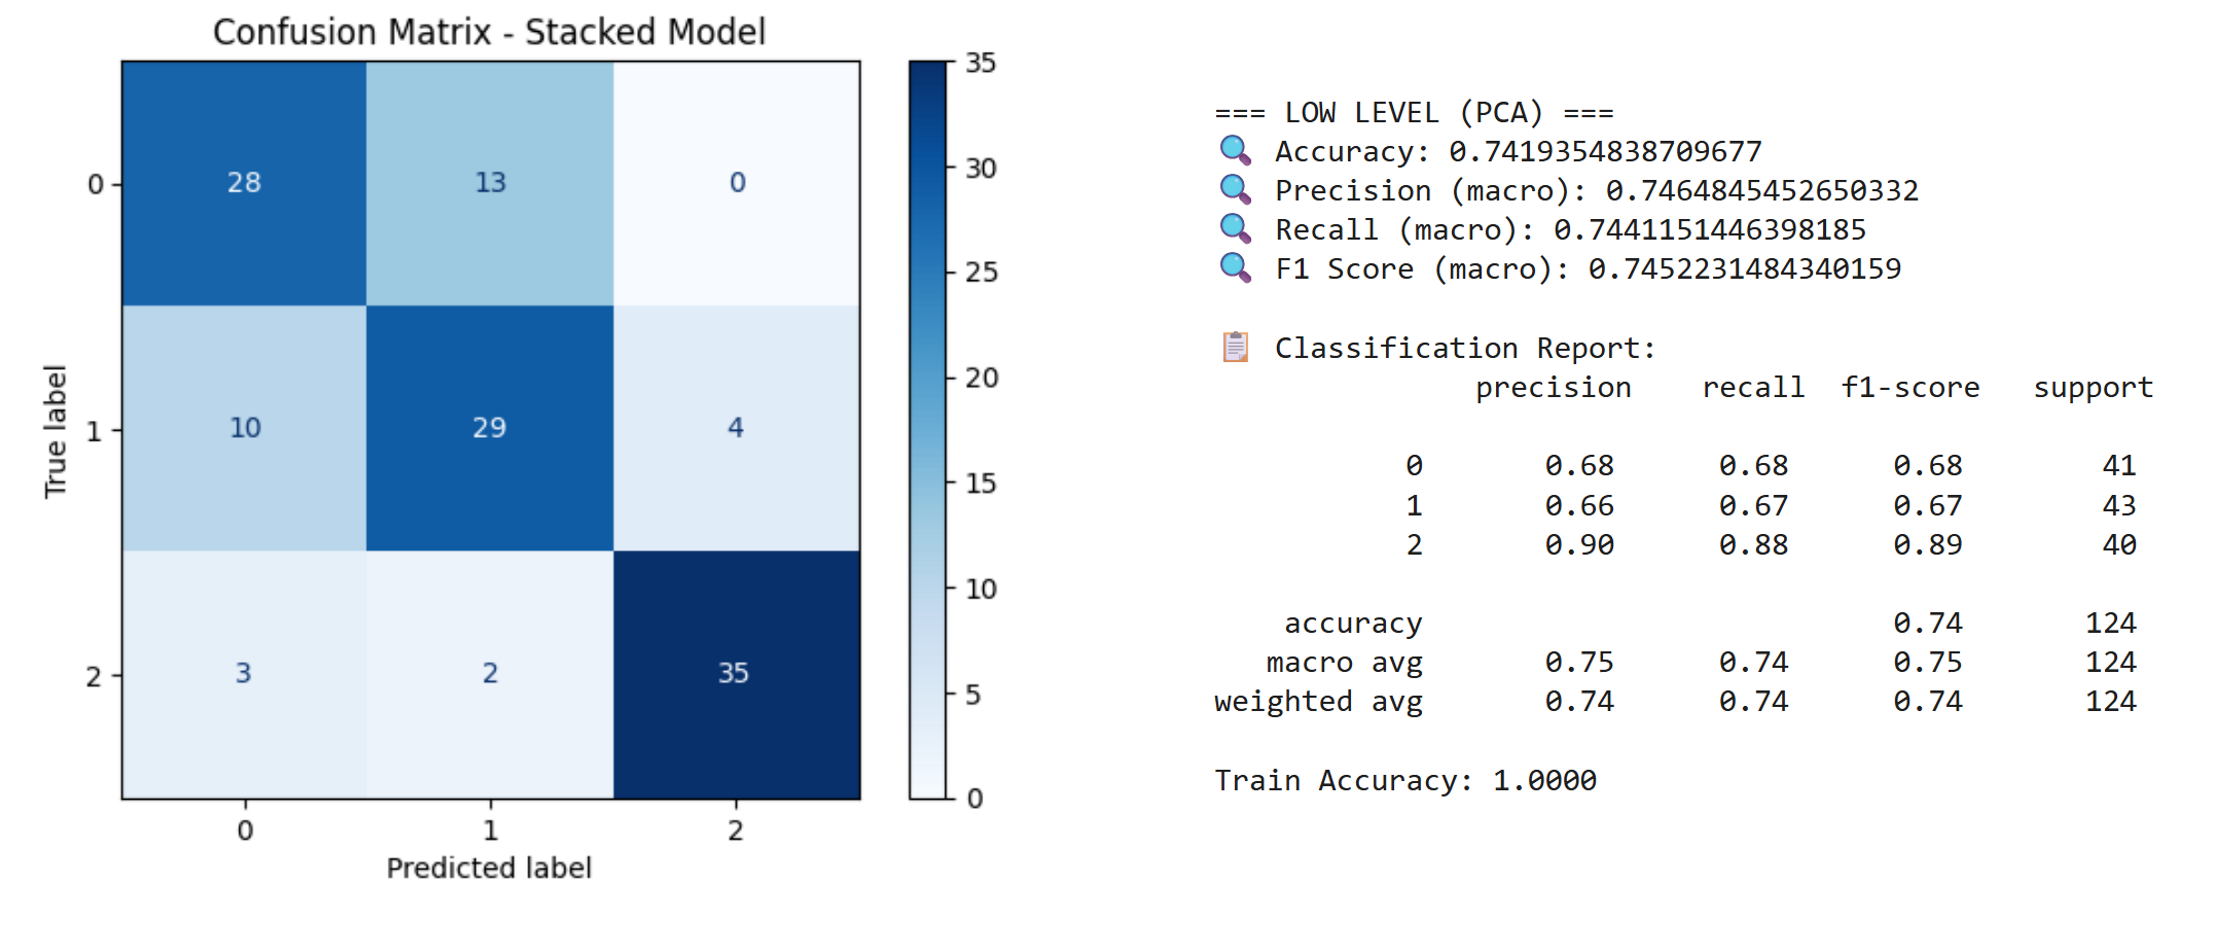
\includegraphics[width=1\textwidth]{1-low.png}
\end{figure}
\FloatBarrier
\begin{figure}[h]
	\centering
	\includegraphics[width=1\textwidth]{1-low2.png}
\end{figure}
\FloatBarrier
\\
نتایج نشان میدهد همچنان ویژگی high بهتر از بقیه عمل میکند. و در دو ویژگی دیگر اورفیت به وجود آمده.و در تمام ویژگی ها کلاس 2 بهتر از بقیه عمل کرده (اسب) که احتمالا به دلیل وجود ویژگی های متمایز بیشتر نسبت به دو گروه دیگر است.
\\
اضافه کردن داده:
\\
\begin{figure}[h]
	\centering
	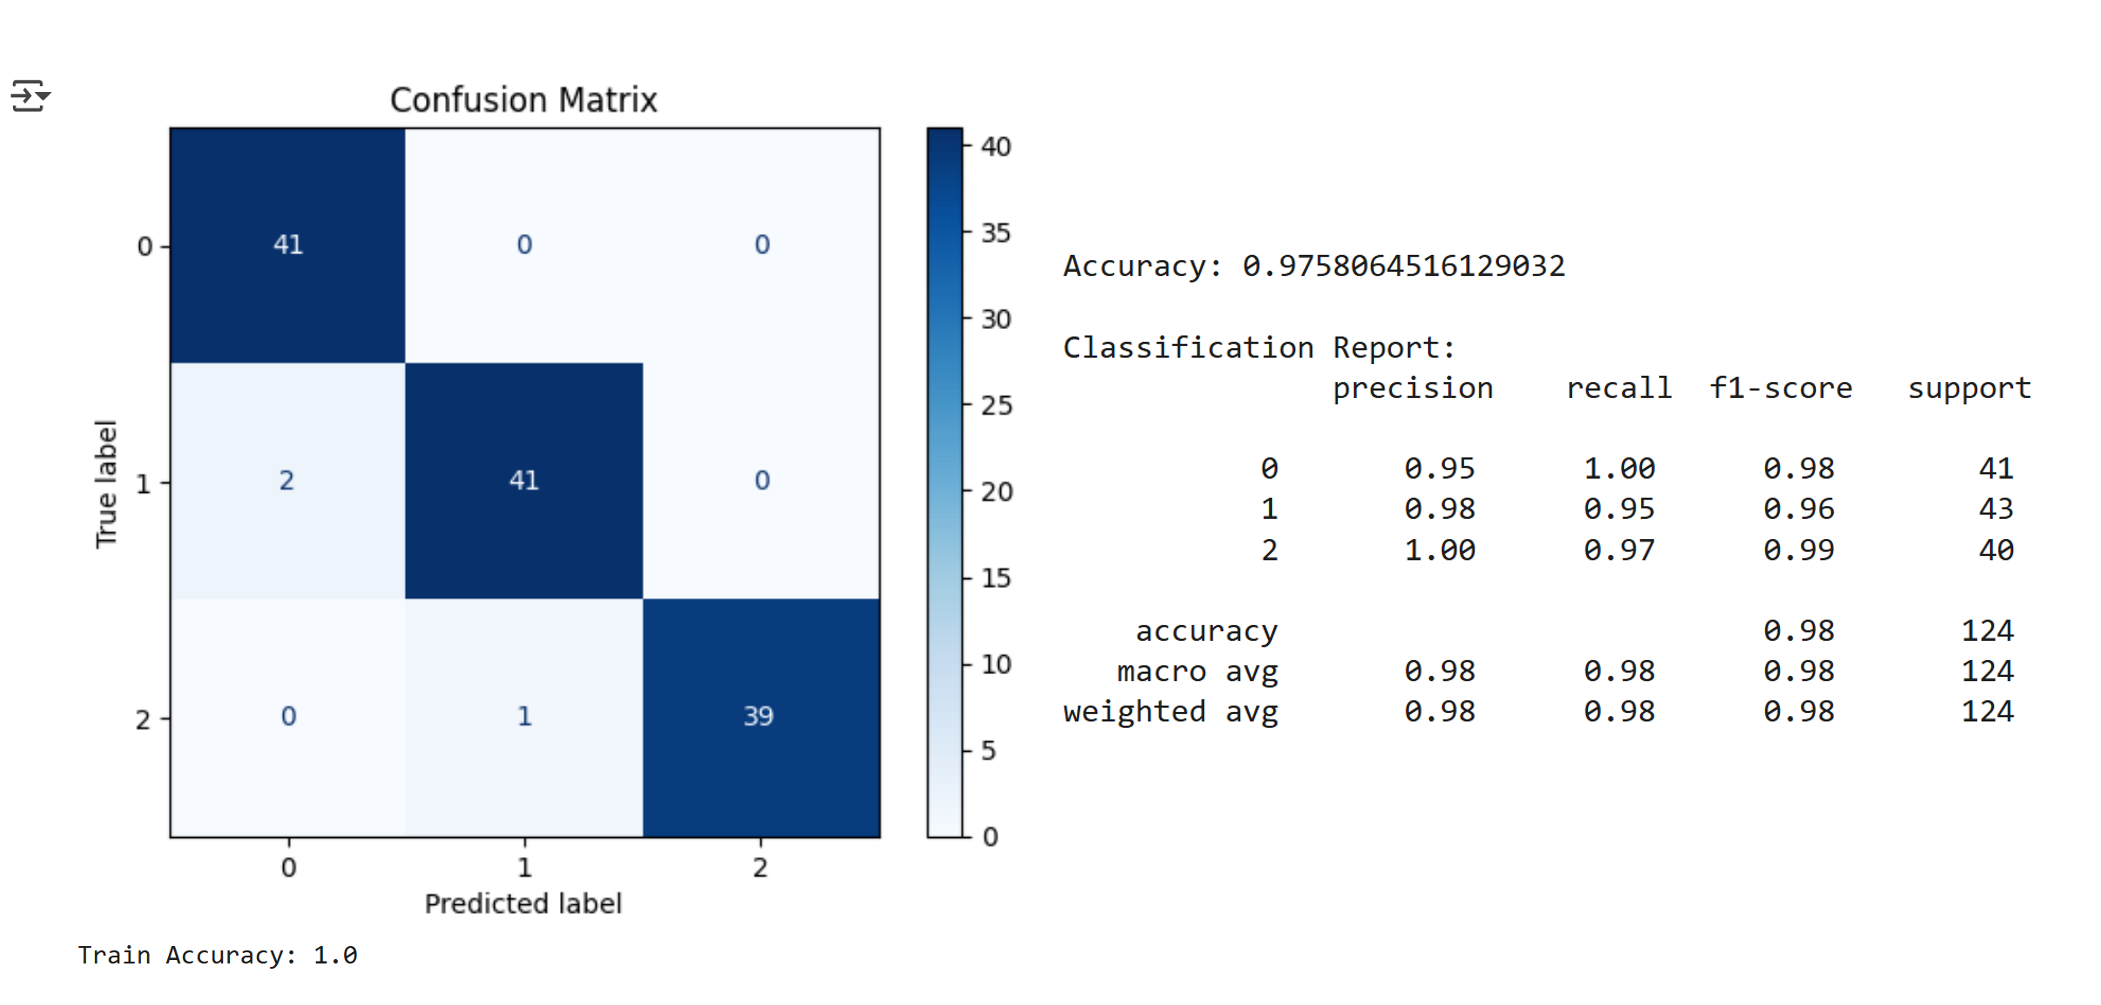
\includegraphics[width=1\textwidth]{2-high.png}
\end{figure}
\FloatBarrier
\begin{figure}[h]
	\centering
	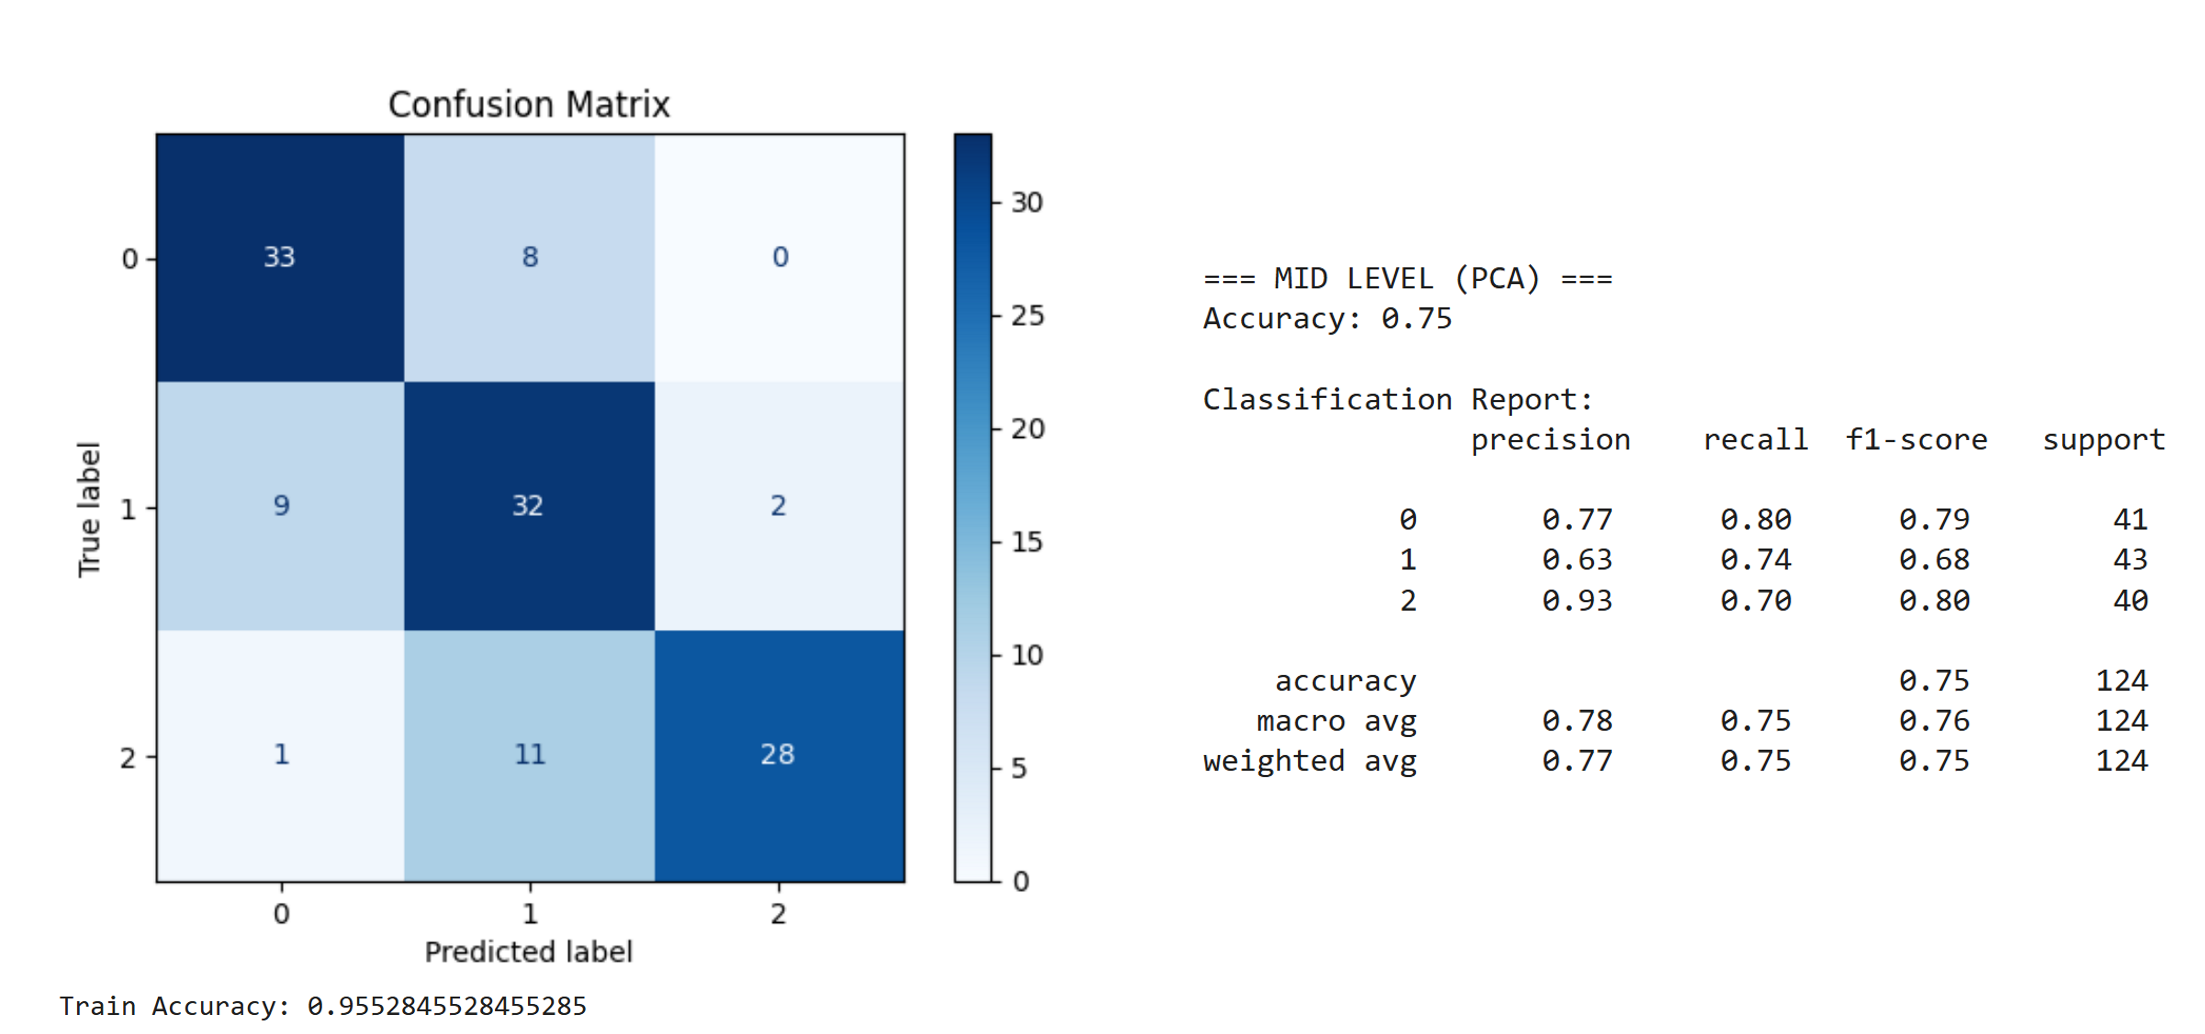
\includegraphics[width=1\textwidth]{2-mid.png}
\end{figure}
\FloatBarrier
\begin{figure}[h]
	\centering
	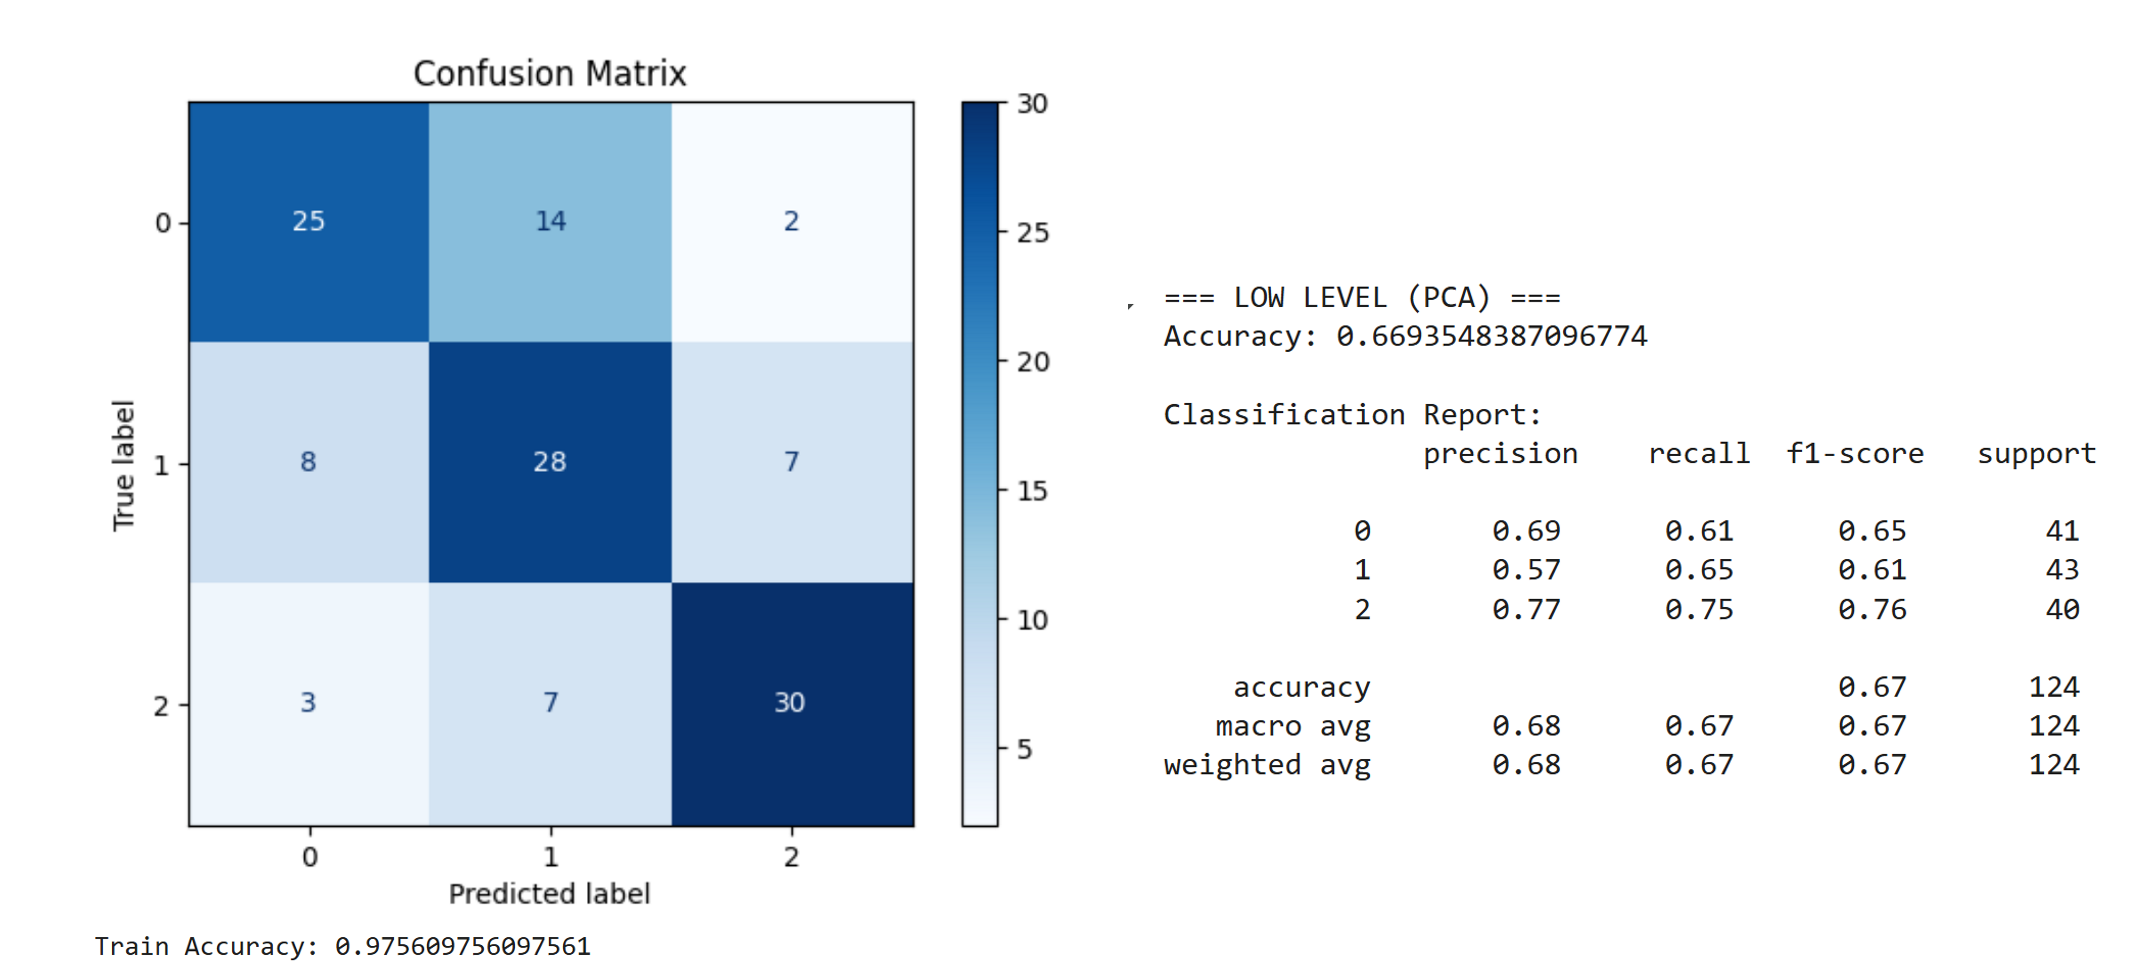
\includegraphics[width=1\textwidth]{2-low.png}
\end{figure}
\FloatBarrier
\\
نتایج نشان می دهد اضافه کردن داده به طور چشمگیری دقت را افزایش نمیدهد ولی کمی در جلوگیری از اورفیت کمک کرده است.
\\
۲. روش دستی (ساخت استک با کنترل بیشتر)\\

در این روش، برخلاف رویکرد کتابخانه‌ای، خودمان فرآیند استکینگ را به‌صورت دستی پیاده‌سازی کردیم. این امر کنترل بیشتری در تنظیم و انتخاب مدل‌ها  به ما داد. در این ساختار، یک یا چند مدل پایه انتخاب شد و خروجی‌های احتمالاتی آن‌ها با استفاده از  \lr{cross val predict}استخراج شده و به مدل نهایی داده شد.
\\
در این روش تنظیمات مدل‌ها دقیق‌تر و هدفمندتر انجام شد.
حتی بدون استفاده از داده افزوده‌شده (Augmentation) نیز دقت تست بالاتری نسبت به روش قبلی حاصل شد.
ساختار طراحی‌شده موجب کاهش اورفیت و افزایش قابلیت تعمیم مدل نهایی شد.
\\
\begin{figure}[h]
	\centering
	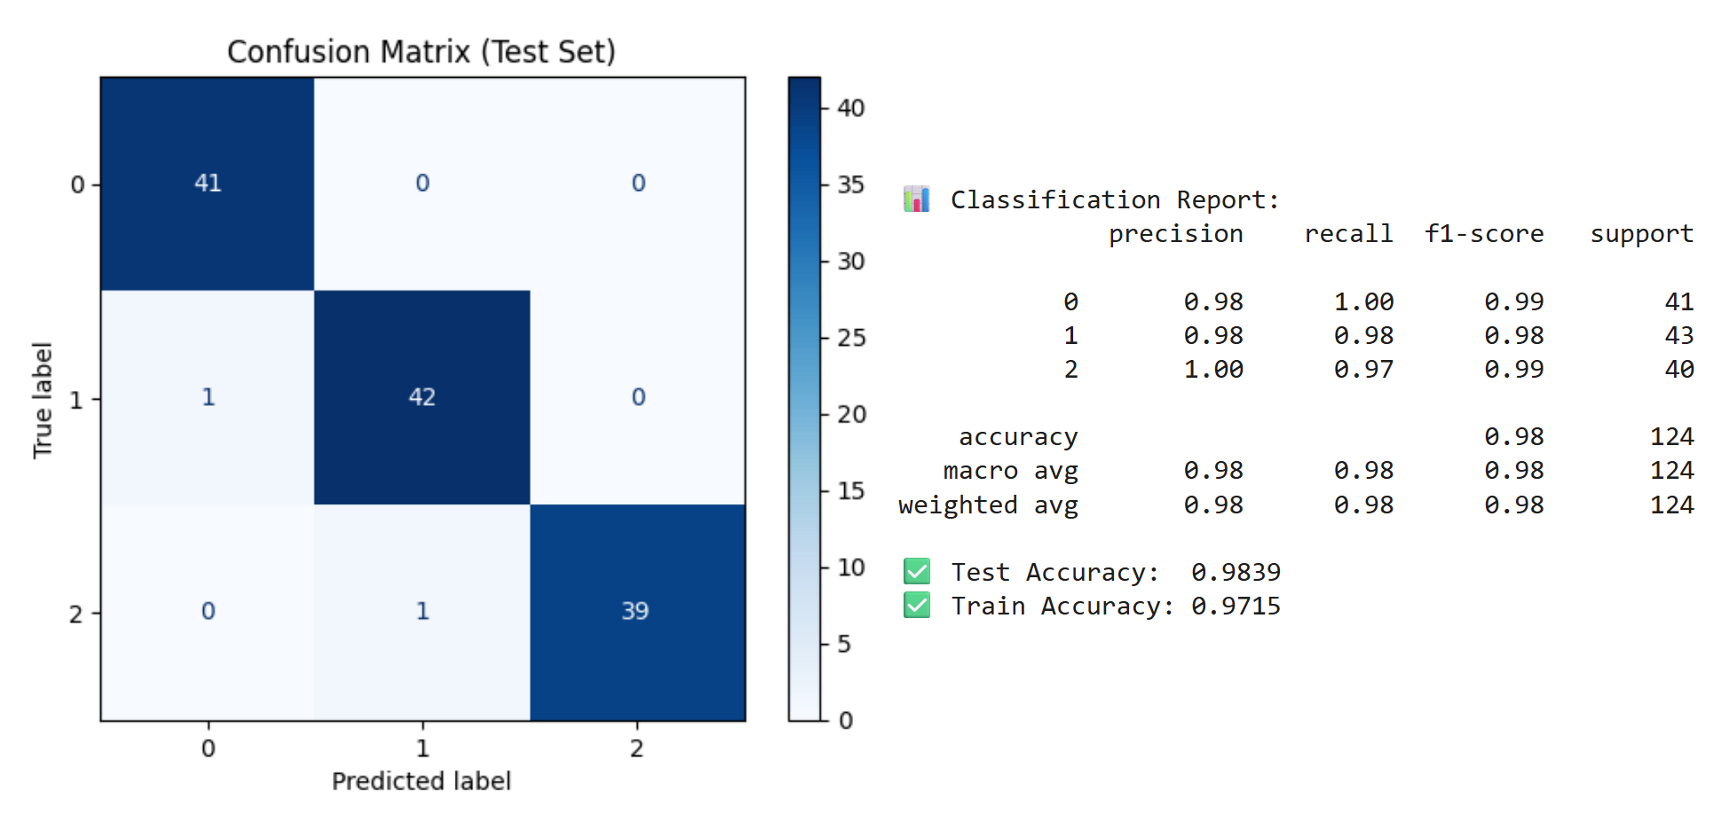
\includegraphics[width=1\textwidth]{3-high.png}
\end{figure}
\FloatBarrier
\begin{figure}[h]
	\centering
	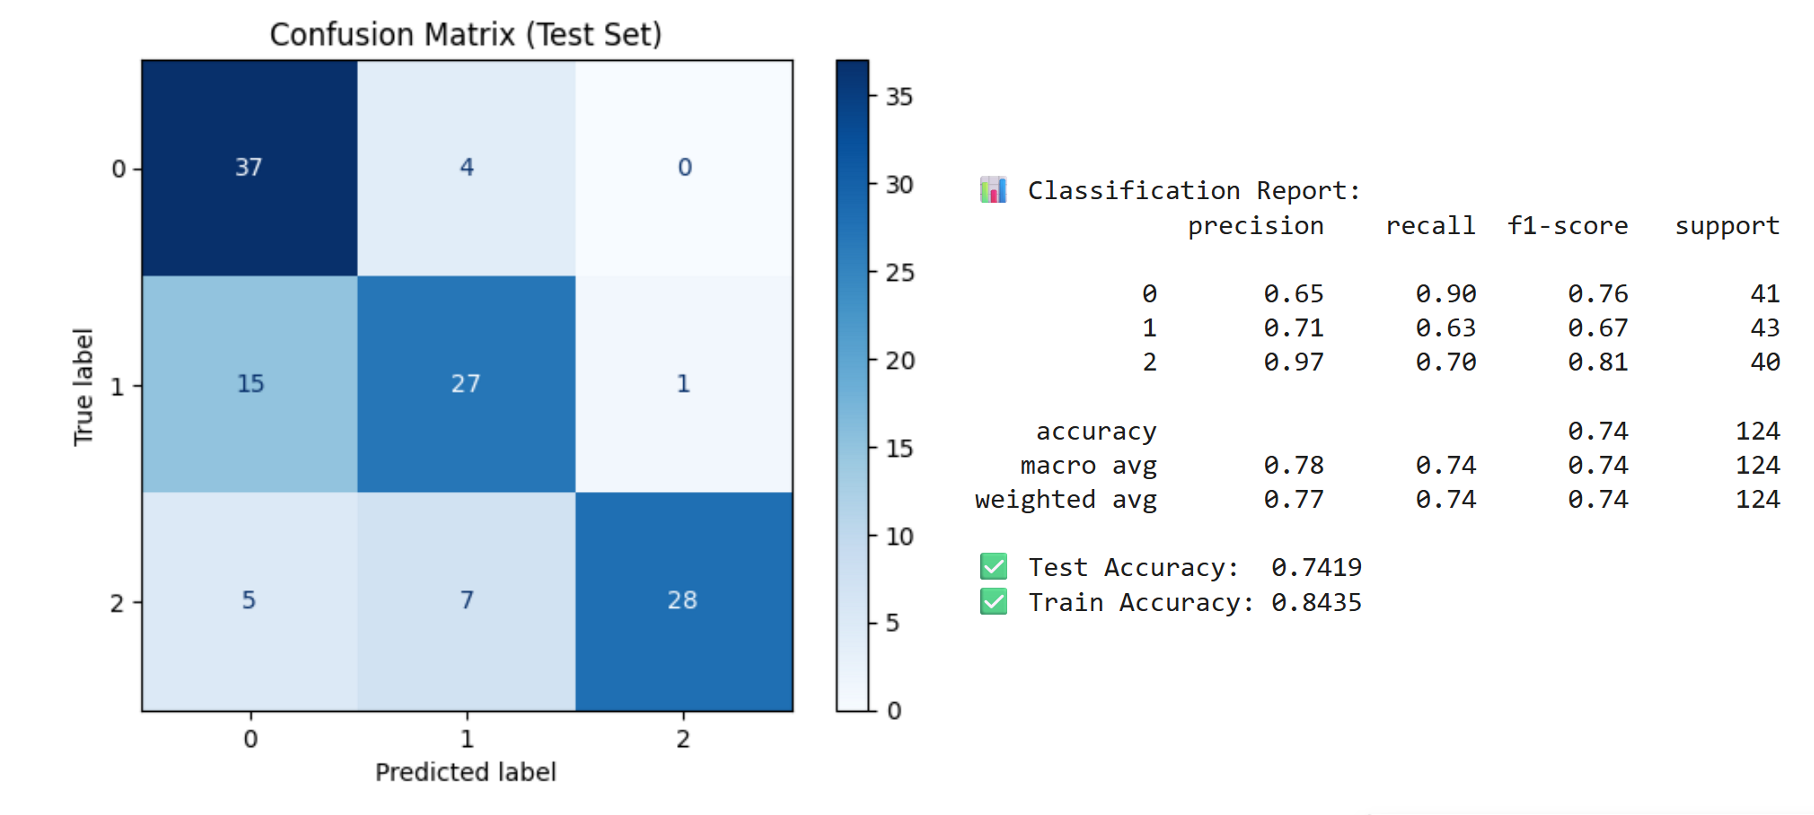
\includegraphics[width=1\textwidth]{3-mid.png}
\end{figure}
\FloatBarrier
\begin{figure}[h]
	\centering
	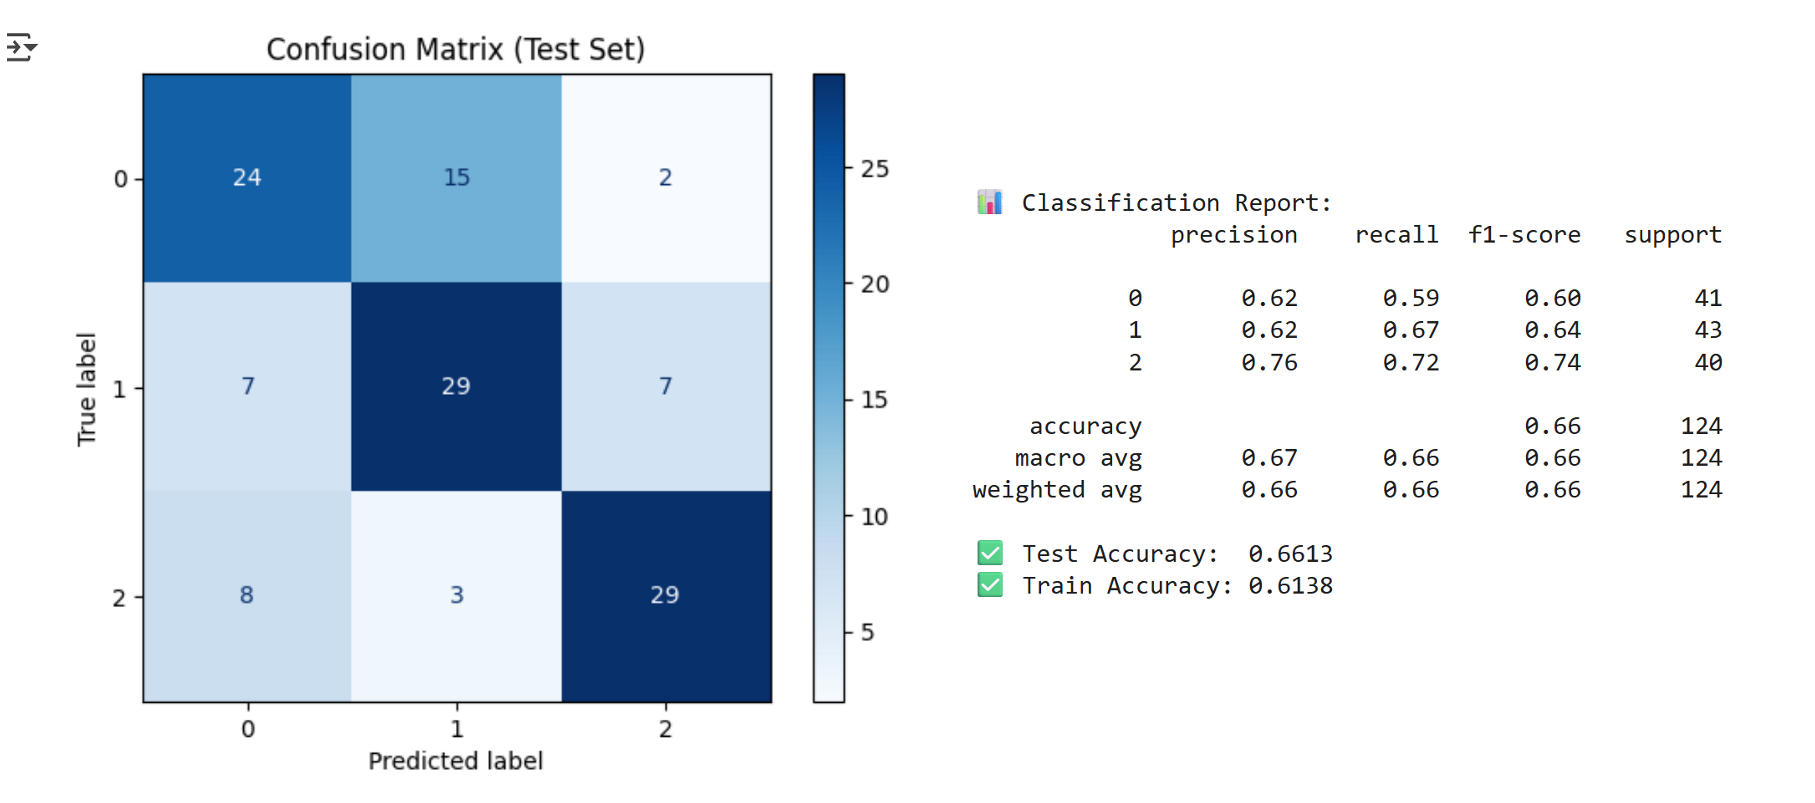
\includegraphics[width=1\textwidth]{3-low.png}
\end{figure}
\FloatBarrier
\\
در اینجا در جلوگیری از اورفیت خیلی بهتر عمل شده و در ویژگی های high همه ی کلاس ها درصد خوبی دارند و در ویژگی mid کلاس 0 بهتر عمل کرده است و در ویژگی low کلاس 1 و 2 بهتر عمل کرده اند.و این نشان میدهد کنترل دستی در کنترل اورفیت کمک بسیاری کرده است
\\
در انتهای این فاز، برای تست نتیجه دو حالت دیگر نیز برای ساخت استک مورد آزمایش قرار گرفت:
\\

استفاده از تمام سطوح ویژگی‌ها به‌طور همزمان به‌عنوان ورودی به مدل نهایی.
\\
\begin{figure}[h]
	\centering
	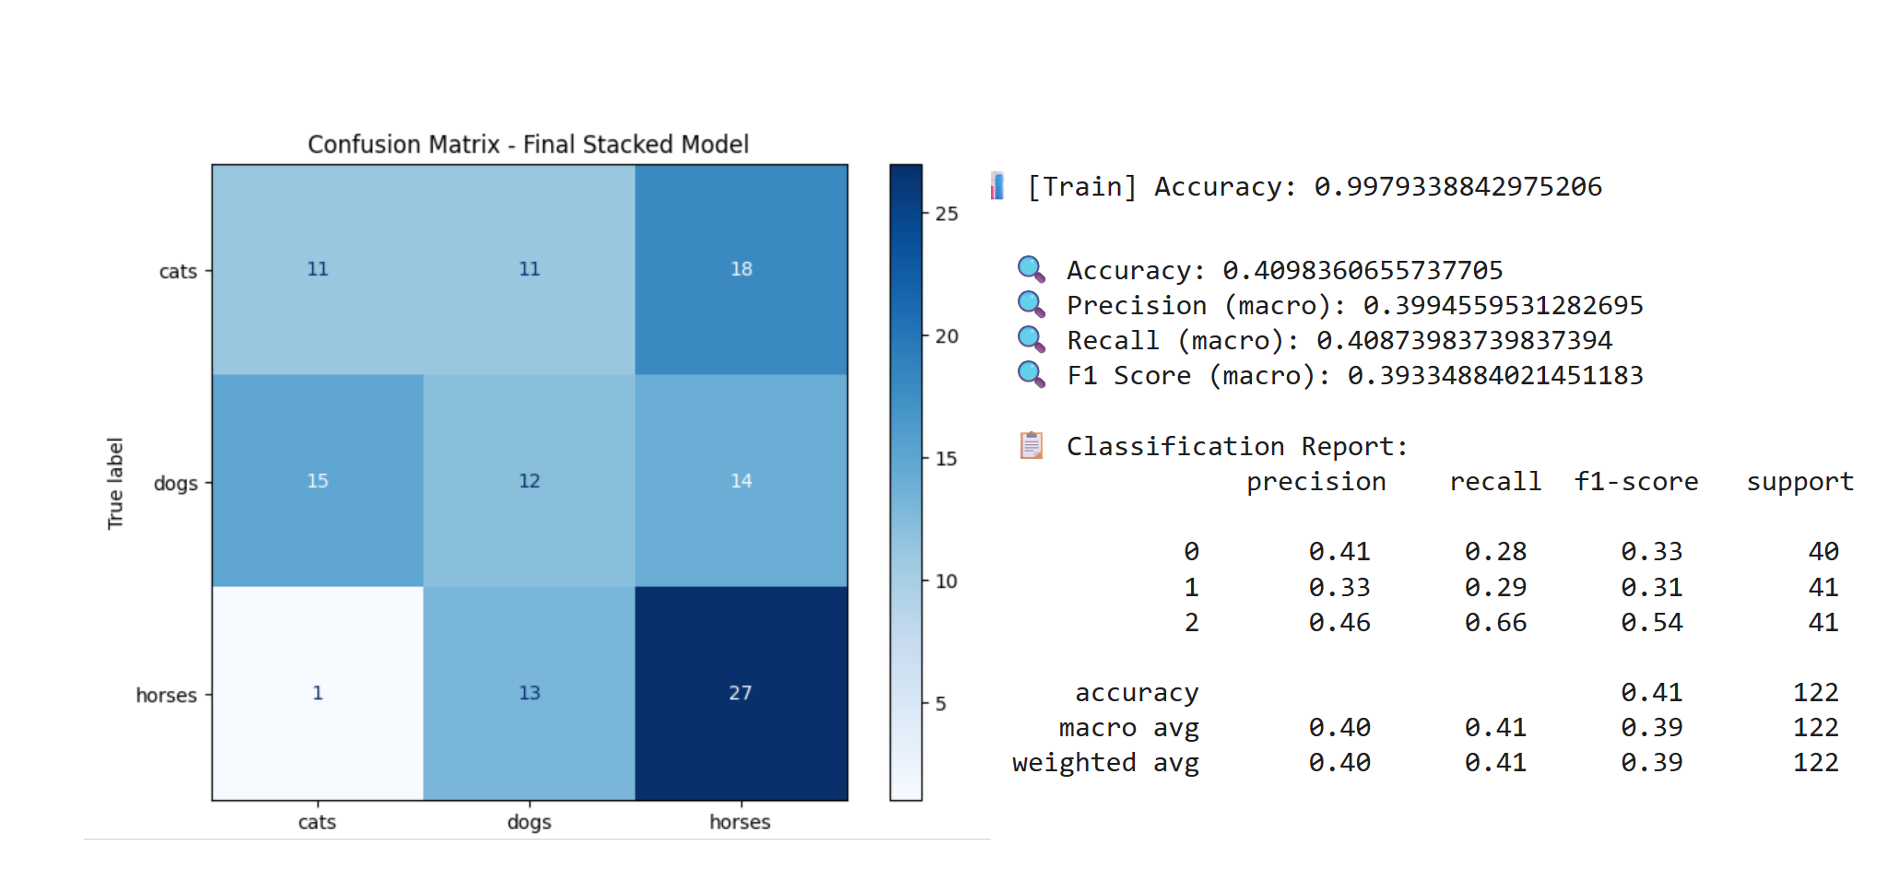
\includegraphics[width=1\textwidth]{all.png}
\end{figure}
\FloatBarrier
\\
ساخت استک ترکیبی با توجه به نتایج فاز اول، به این صورت که از هر سطح ویژگی، فقط بهترین مدل طبقه‌بند (با توجه به دقت فاز قبلی) انتخاب شده و در استک نهایی استفاده گردید.
\\
\begin{figure}[h]
	\centering
	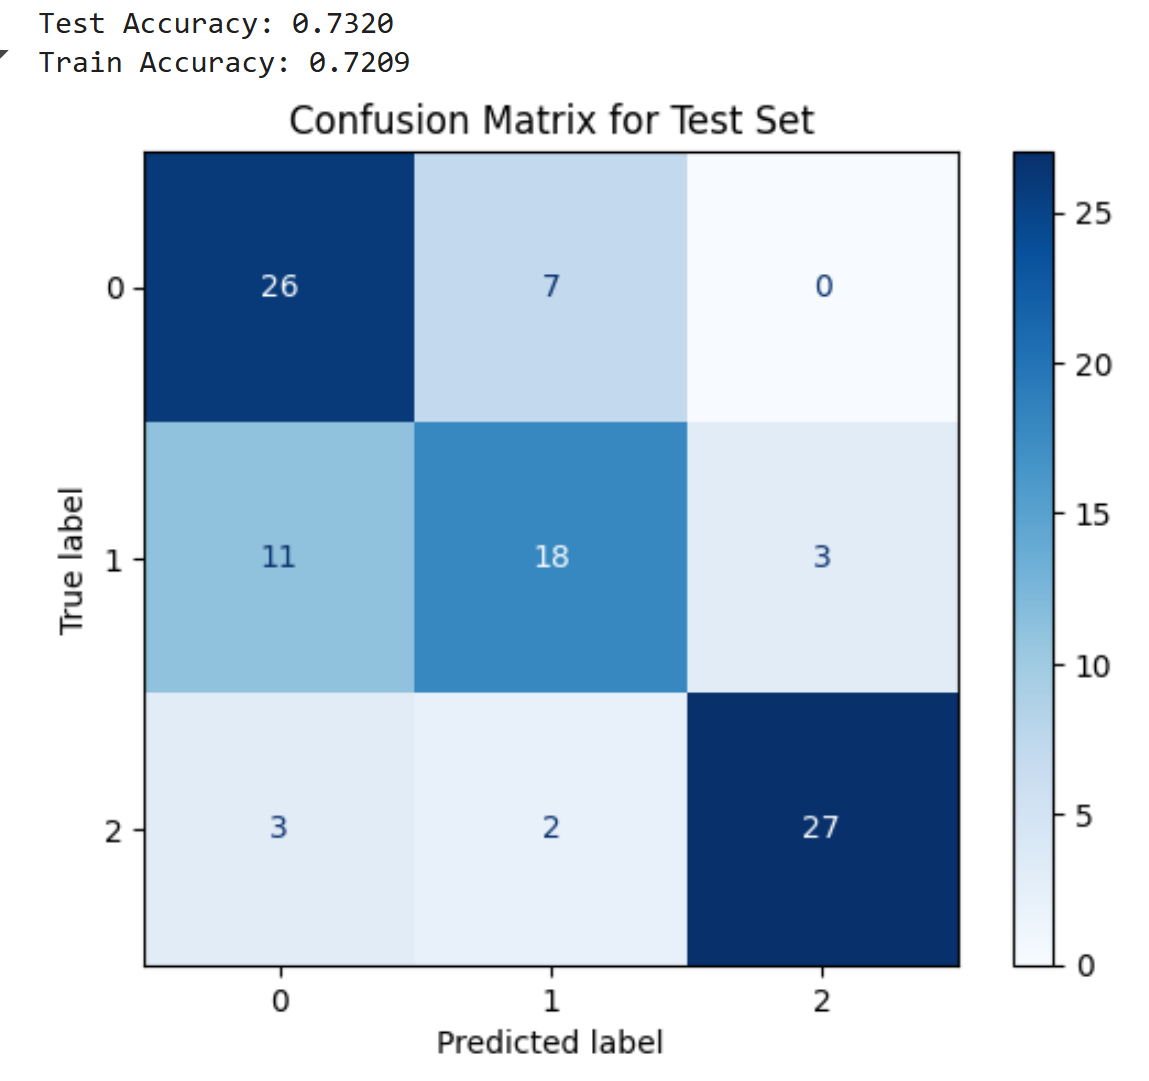
\includegraphics[width=1\textwidth]{tarkib.png}
\end{figure}
\FloatBarrier
\\
نتایج نشان دادند که حالت دوم (ترکیبی و انتخابی) به مراتب ساده‌تر، سریع‌تر و با عملکرد مشابه یا بهتر نسبت به حالت اول عمل کرده است.\\
\\
 چرا  High-Level Feature خیلی خوب کار کرد؟\\
 چون Highlevel  لایه‌های آخر شبکه هستند و اطلاعات انتزاعی و معنایی تصویر را بهتر درک کرده‌اند (مثل شکل، کلاس، بافت‌های متمایز). Mid و Low  بیشتر ویژگی‌های اولیه را استخراج می‌کنند (مانند لبه‌ها، رنگ‌ها، بافت ساده) که به تنهایی برای تفکیک کلاس‌های پیچیده کافی نیستند.
\\
برای جلوگیری از اورفیت شدن هم از اضافه کردن دیتا (برای افزایش تنوع داده) استفاده کردیم  و هم از pca برای کاهش ابعاد ویژگی ها تا به صورت کلی تر کار کنند و به داده ی آموزشی زیاد وابسته نباشند
\\
مقایسه با فاز یک:
\\
در استفاده از استک مدل‌های مختلف دیدگاه‌های مختلفی به داده دارند. مثلاً:

SVM ممکنه برای داده‌های با مرزهای واضح بهتر باشه،
\\
Random Forest برای داده‌های نویزی و پیچیده،
\\
Naive Bayes برای فرض استقلال ویژگی‌ها.
\\
استکینگ همه‌ی این دیدگاه‌ها رو با هم ترکیب می‌کنه و یک تصمیم نهایی هوشمندانه‌تر می‌گیره.
\\
همچنین هر مدل پایه ممکنه در تشخیص برخی کلاس‌ها یا انواع خاصی از نمونه‌ها ضعیف باشه. وقتی خروجی چند مدل به مدل نهایی داده میشه: مدل متا (مثلاً Logistic Regression در استک) یاد می‌گیره کِی به کدوم مدل بیشتر اعتماد کنه. مثلاً اگر "اگه MLP گفته است کلاس 2 و بقیه شک داشتند، احتمال زیاد درست است".
\\
استکینگ با استفاده از cross-validation روی مدل‌های پایه، جلوی اورفیت کردن به یک مدل خاص رو می‌گیره. در واقع به جای اینکه از یک مدل استفاده کند ،از خروجی چند مدل با هم استفاده می‌کند، و مدل نهایی تصمیم می‌گیره کدام مهم تر است.
\\
همچنین می شود چون سه سطح ویژگی مختلف (low/mid/high) داریم،  از استکینگ به صورت ترکیبی استفاده کنیم از MLP روی ویژگی‌های high،از SVM روی ویژگی‌های mid، و از Logistic Regression روی ویژگی‌های low
استفاده کند، و همه‌ی خروجی‌ها رو ترکیب کند.
\\
 Stacking اغلب:
از هر مدل پایه به‌تنهایی بهتر عمل می‌کنه،
به‌ویژه در دیتاست‌های پیچیده و چندکلاسه. در اینجا هم نتایج فاز دوم ( مخصوصا قسمت تنظیم دستی) از تک تک موارد فاز اول بهتر بوده است و در ویژگی های high همیشه خوب عمل شده  و در دو ویژگی دیگر از بهترین فاز اول یا هم اندازه یا بهتر عمل کرده است
\end{document} 